\let\ifdeutsch\iffalse
\let\ifenglisch\iftrue
% EN: This file is loaded before the \documentclass command in the main document

% EN: The following package allows \\ at the title page
%     For more information see https://github.com/latextemplates/scientific-thesis-cover/issues/4
\RequirePackage{kvoptions-patch}

\ifenglisch
  \PassOptionsToClass{numbers=noenddot}{scrbook}
\else
  %()Aus scrguide.pdf - der Dokumentation von KOMA-Script)
  %Nach DUDEN steht in Gliederungen, in denen ausschließlich arabische Ziffern für die Nummerierung
  %verwendet werden, am Ende der Gliederungsnummern kein abschließender Punkt
  %(siehe [DUD96, R3]). Wird hingegen innerhalb der Gliederung auch mit römischen Zahlen
  %oder Groß- oder Kleinbuchstaben gearbeitet, so steht am Ende aller Gliederungsnummern ein
  %abschließender Punkt (siehe [DUD96, R4])
  \PassOptionsToClass{numbers=autoendperiod}{scrbook}
\fi

% Warns about outdated packages and missing caption declarations
% See https://www.ctan.org/pkg/nag
\RequirePackage[l2tabu, orthodox]{nag}

%DE: Neue deutsche Trennmuster
%    Siehe http://www.ctan.org/pkg/dehyph-exptl und http://projekte.dante.de/Trennmuster/WebHome
%    Nur für pdflatex, nicht für lualatex
\RequirePackage{ifluatex}
\ifluatex
  % do not load anything
\else
  \ifdeutsch
    \RequirePackage[ngerman=ngerman-x-latest]{hyphsubst}
  \fi
\fi

\documentclass[
  fontsize=12pt,
  a4paper,  % Standard format - only KOMAScript uses paper=a4 - https://tex.stackexchange.com/a/61044/9075
  twoside,  % we are optimizing for both screen and two-side printing. So the page numbers will jump, but the content is configured to stay in the middle (by using the geometry package)
  bibliography=totoc,
  %listof=totoc, %to add list of figures to toc
  %               idxtotoc,   %Index ins Inhaltsverzeichnis
  %               liststotoc, %List of X ins Inhaltsverzeichnis, mit liststotocnumbered werden die Abbildungsverzeichnisse nummeriert
  headsepline,
  cleardoublepage=empty,
  %               draft    % um zu sehen, wo noch nachgebessert werden muss - wichtig, da Bindungskorrektur mit drin
  draft=false
]{scrbook}
% !TeX encoding = utf8
% -*- coding:utf-8 mod:LaTeX -*-

% EN: This file includes basic packages and sets options. The order of package
%     loading is important

% DE: In dieser Datei werden zuerst die benoetigten Pakete eingebunden und
%     danach diverse Optionen gesetzt. Achtung Reihenfolge ist entscheidend!


% EN: Styleguide:
% - English comments are prefixed with "EN", German comments are prefixed with "DE"
% - Prefixed headings define the language for the subsequent paragraphs
% - It is tried to organize packages in blocks. Bocks are separated by two empty lines.

% DE: Styleguide:
%
% Ein sehr kleiner Styleguide. Packages werden in Blöcken organisiert.
% Zwischen zwei Blöcken sind 2 Leerzeilen!


% EN: Enable copy and paste of text from the PDF
%     Only required for pdflatex. It "just works" in the case of lualatex.
%     mmap enables mathematical symbols, but does not work with the newtx font set
%     See: https://tex.stackexchange.com/a/64457/9075
%     Other solutions outlined at http://goemonx.blogspot.de/2012/01/pdflatex-ligaturen-und-copynpaste.html and http://tex.stackexchange.com/questions/4397/make-ligatures-in-linux-libertine-copyable-and-searchable
%     Trouble shooting outlined at https://tex.stackexchange.com/a/100618/9075

\ifluatex
\else
  \usepackage{cmap}
\fi


% EN: File encoding
% DE: Codierung
%     Wir sind im 21 Jahrhundert, utf-8 löst so viele Probleme.
%
% Mit UTF-8 funktionieren folgende Pakete nicht mehr. Bitte beachten!
%   * fancyvrb mit §
%   * easylist -> http://www.ctan.org/tex-archive/macros/latex/contrib/easylist/
\ifluatex
  % EN: See https://tex.stackexchange.com/a/158517/9075
  %     Not required, because of usage of fontspec package
  %\usepackage[utf8]{luainputenc}
\else
  \usepackage[utf8]{inputenc}
\fi


% DE: Parallelbetrieb tex4ht und pdflatex

\makeatletter
\@ifpackageloaded{tex4ht}{
  \def\iftex4ht{\iftrue}
}{
  \def\iftex4ht{\iffalse}
}
\makeatother


% EN: Mathematics
% DE: Mathematik
%
% DE: Viele Mathematik-Sachen. Siehe https://texdoc.net/pkg/amsmath
%
% EN: Options must be passed this way, otherwise it does not work with glossaries
% DE: fleqn (=Gleichungen linksbündig platzieren) funktioniert nicht direkt. Es muss noch ein Patch gemacht werden:
\PassOptionsToPackage{fleqn,leqno}{amsmath}
%
% DE: amsmath Muss nicht mehr geladen werden, da es von newtxmath automatisch geladen wird
% \usepackage{amsmath}


%% EN: Fonts
%% DE: Schriften
%%
%% !!! If you change the font, be sure that words such as "workflow" can
%% !!! still be copied from the PDF. If this is not the case, you have
%% !!! to use glyphtounicode. See comment at cmap package


% EN: Times Roman for all text
\ifluatex
  % source: Second proposed fix from the following answer: https://tex.stackexchange.com/a/394137
  \usepackage[no-math]{fontspec}
  \setmainfont{TeXGyreTermes-Regular}[
       BoldFont       = TeXGyreTermes-Bold ,
       ItalicFont     = TeXGyreTermes-Italic ,
       BoldItalicFont = TeXGyreTermes-BoldItalic,
       NFSSFamily     = ntxtlf]
  \setsansfont{TeX Gyre Heros Regular}[
       Scale=.9,
       BoldFont       = TeX Gyre Heros Bold,
       ItalicFont     = TeX Gyre Heros Italic,
       BoldItalicFont = TeX Gyre Heros BoldItalic]
  \setmonofont[StylisticSet={1,3},Scale=.9]{inconsolata}
  \RequirePackage{newtxmath}
\else
  \RequirePackage{newtxtext}
  \RequirePackage{newtxmath}
  % EN: looks good with times, but no equivalent for lualatex found,
  %     therefore replaced with inconsolata
  %\RequirePackage[zerostyle=b,scaled=.9]{newtxtt}
  \RequirePackage[varl,scaled=.9]{inconsolata}
\fi

% EN: Fallback font - if the subsequent font packages do not define a font (e.g., monospaced)
%     This is the modern package for "Computer Modern".
%     In case this gets activated, one has to switch from cmap package to glyphtounicode (in the case of pdflatex)
% DE: Fallback-Schriftart
%\usepackage[%
%    rm={oldstyle=false,proportional=true},%
%    sf={oldstyle=false,proportional=true},%
%    tt={oldstyle=false,proportional=true,variable=true},%
%    qt=false%
%]{cfr-lm}

% EN: Headings are typset in Helvetica (which is similar to Arial)
% DE: Schriftart fuer die Ueberschriften - ueberschreibt lmodern
%\usepackage[scaled=.95]{helvet}

% DE: Für Schreibschrift würde tun, muss aber nicht
%\usepackage{mathrsfs} %  \mathscr{ABC}

% EN: Font for the main text
% DE: Schriftart fuer den Fliesstext - ueberschreibt lmodern
%     Linux Libertine, siehe http://www.linuxlibertine.org/
%     Packageparamter [osf] = Minuskel-Ziffern
%     rm = libertine im Brottext, Linux Biolinum NICHT als serifenlose Schrift, sondern helvet (von oben) beibehalten
%\usepackage[rm]{libertine}

% EN: Alternative Font: Palantino. It is recommeded by Prof. Ludewig for German texts
% DE: Alternative Schriftart: Palantino, Packageparamter [osf] = Minuskel-Ziffern
%     Bitte nur in deutschen Texten
%\usepackage{mathpazo} %ftp://ftp.dante.de/tex-archive/fonts/mathpazo/ - Tipp aus DE-TEX-FAQ 8.2.1

% DE: Schriftart fuer Programmcode - ueberschreibt lmodern
%     Falls auskommentiert, wird die Standardschriftart lmodern genommen
%     Fuer schreibmaschinenartige Schluesselwoerter in den Listings - geht bei alten Installationen nicht, da einige Fontshapes (<>=) fehlen
%\usepackage[scaled=.92]{luximono}
%\usepackage{courier}
% DE: BeraMono als Typewriter-Schrift, Tipp von http://tex.stackexchange.com/a/71346/9075
%\usepackage[scaled=0.83]{beramono}

% EN: backticks (`) are rendered as such in verbatim environments.
%     See following links for details:
%     - https://tex.stackexchange.com/a/341057/9075
%     - https://tex.stackexchange.com/a/47451/9075
%     - https://tex.stackexchange.com/a/166791/9075
\usepackage{upquote}

% DE: Symbole
%
%\usepackage[geometry]{ifsym} % \BigSquare
%\usepackage{mathabx}
%\usepackage{stmaryrd} %fuer \ovee, \owedge, \otimes
%\usepackage{marvosym} %fuer \Writinghand %patched to not redefine \Rightarrow
%\usepackage{mathrsfs} %mittels \mathscr{} schoenen geschwungenen Buchstaben erzeugen
%\usepackage{calrsfs} %\mathcal{} ein bisserl dickeren buchstaben erzeugen - sieht net so gut aus.
%durch mathpazo ist das schon definiert

%
%\usepackage{amssymb}

% EN: For \texttrademark{}
\usepackage{textcomp}

% EN: name-clashes von marvosym und mathabx vermeiden:
\def\delsym#1{%
  %  \expandafter\let\expandafter\origsym\expandafter=\csname#1\endcsname
  %  \expandafter\let\csname orig#1\endcsname=\origsym
  \expandafter\let\csname#1\endcsname=\relax
}

%\usepackage{pifont}
%\usepackage{bbding}
%\delsym{Asterisk}
%\delsym{Sun}\delsym{Mercury}\delsym{Venus}\delsym{Earth}\delsym{Mars}
%\delsym{Jupiter}\delsym{Saturn}\delsym{Uranus}\delsym{Neptune}
%\delsym{Pluto}\delsym{Aries}\delsym{Taurus}\delsym{Gemini}
%\delsym{Rightarrow}
%\usepackage{mathabx} - Ueberschreibt leider zu viel - und die \le-Zeichen usw. sehen nicht gut aus!


% EN: Modern font encoding
%     Has to be loaded AFTER any font packages. See https://tex.stackexchange.com/a/2869/9075.
\ifluatex
\else
  \usepackage[T1]{fontenc}
\fi
%


% EN: Character protrusion and font expansion. See http://www.ctan.org/tex-archive/macros/latex/contrib/microtype/
% DE: Optischer Randausgleich und Grauwertkorrektur

\usepackage[
  babel=true, % EN: Enable language-specific kerning. Take language-settings from the languge of the current document (see Section 6 of microtype.pdf)
  expansion=alltext,
  protrusion=alltext-nott, % EN: Ensure that at listings, there is no change at the margin of the listing
  final % EN: Always enable microtype, even if in draft mode. This helps finding bad boxes quickly.
        %     In the standard configuration, this template is always in the final mode, so this option only makes a difference if "pros" use the draft mode
]{microtype}


% EN: \texttt{test -- test} keeps the "--" as "--" (and does not convert it to an en dash)
\DisableLigatures{encoding = T1, family = tt* }

% DE: fuer microtype
% DE: tracking=true muss als Parameter des microtype-packages mitgegeben werden
% DE: Deaktiviert, da dies bei Algorithmen seltsam aussieht

%\DeclareMicrotypeSet*[tracking]{my}{ font = */*/*/sc/* }%
%\SetTracking{ encoding = *, shape = sc }{ 45 }
% DE: Hier wird festgelegt,
%     dass alle Passagen in Kapitälchen automatisch leicht
%     gesperrt werden.
%     Quelle: http://homepage.ruhr-uni-bochum.de/Georg.Verweyen/pakete.html
%    Deaktiviert, da sonst "BPEL", "BPMN" usw. wirklich komisch aussehen.
%     Macht wohl nur bei geisteswissenschaftlichen Arbeiten Sinn.


% EN: amsmath teaks


% EN: Fixes bugs in AMS math
%     Corrently conflicts with unicode-math
% \usepackage{mathtools}

%\numberwithin{equation}{section}
%\renewcommand{\theequation}{\thesection.\Roman{equation}}

% EN: work-around ams-math problem with align and 9 -> 10. Does not work with glossaries, No visual changes.
%\addtolength\mathindent{1em}


% EN: For theorems, replacement for amsthm
\usepackage[amsmath,hyperref]{ntheorem}
\theorempreskipamount 2ex plus1ex minus0.5ex
\theorempostskipamount 2ex plus1ex minus0.5ex
\theoremstyle{break}
\newtheorem{definition}{Definition}[section]


% CTAN: https://ctan.org/pkg/lccaps
% Doc: http://texdoc.net/pkg/lccaps
%
% Required for DE/EN \initialism
\usepackage{lccaps}


% EN: Defintion of colors. Argument "hyperref" is not used as we do not want to change border colors of links: Links are not colored anymore.
% DE: Farbdefinitionen
\usepackage[dvipsnames]{xcolor}


% EN: Required for custom acronyms/glossaries style.
%     Left aligned Columns in tables with fixed width.
%     See http://tex.stackexchange.com/questions/91566/syntax-similar-to-centering-for-right-and-left
\usepackage{ragged2e}


% DE: Wichtig, ansonsten erscheint "No room for a new \write"
\usepackage{scrwfile}


% EN: Support for language-specific hyphenation
% DE: Neue deutsche Rechtschreibung und Literatur statt "Literature"
%     Die folgende Einstellung ist der Nachfolger von ngerman.sty
\ifdeutsch
  % DE: letzte Sprache ist default, Einbindung von "american" ermöglicht \begin{otherlanguage}{amercian}...\end{otherlanguage} oder \foreignlanguage{american}{Text in American}
  %     Siehe auch http://tex.stackexchange.com/a/50638/9075
  \usepackage[american,main=ngerman]{babel}
  % Ein "abstract" ist eine "Kurzfassung", keine "Zusammenfassung"
  \addto\captionsngerman{%
    \renewcommand\abstractname{Kurzfassung}%
  }
  \ifluatex
    % EN: conditionally disable ligatures. See https://github.com/latextemplates/scientific-thesis-template/issues/54
    %     for a discussion
    \usepackage[ngerman]{selnolig}
  \fi
\else
  % EN: Set English as language and allow to write hyphenated"=words
  %     `american`, `english` and `USenglish` are synonyms for babel package (according to https://tex.stackexchange.com/questions/12775/babel-english-american-usenglish).
  %      "english" has to go last to set it as default language
  \usepackage[ngerman,main=english]{babel}
  % EN: Hint by http://tex.stackexchange.com/a/321066/9075 -> enable "= as dashes
  \addto\extrasenglish{\languageshorthands{ngerman}\useshorthands{"}}
  \ifluatex
    % EN: conditionally disable ligatures. See https://github.com/latextemplates/scientific-thesis-template/issues/54
    %     for a discussion
    \usepackage[english]{selnolig}
  \fi
\fi
%


% EN: For easy quotations: \enquote{text}
%     This package is very smart when nesting is applied, otherwise textcmds (see below) provides a shorter command
%     Note that this package results in a warning when it is loaded before minted (actually fvextra).
% DE: Anführungszeichen
%     Zitate in \enquote{...} setzen, dann werden automatisch die richtigen Anführungszeichen verwendet.
%     Dieses package erzeugt eine Warnung, wenn es vor minted (genauer fvextra) geladen wird.
\usepackage{csquotes}


% EN: For even easier quotations: \qq{text}.
%     Is not smart in the case of nesting, but good enough for the most cases
\usepackage{textcmds}
\ifdeutsch
  % EN: German quotes are different. So do not use the English quotes, but the ones provided by the csquotes package.
  \renewcommand{\qq}[1]{\enquote{#1}}
\fi


% EN: extended enumarations
% DE: erweitertes Enumerate
\usepackage{paralist}


% DE: Gestaltung der Kopf- und Fußteilen

\usepackage[automark]{scrlayer-scrpage}

\automark[section]{chapter}
\setkomafont{pageheadfoot}{\normalfont\sffamily}
\setkomafont{pagenumber}{\normalfont\sffamily}

% DE: funktioniert nicht: Alle Linien sind hier weg
%\setheadsepline[.4pt]{.4pt}


% DE: Intelligentes Leerzeichen um hinter Abkürzungen die richtigen Abstände zu erhalten, auch leere.
%     Siehe commands.tex \gq{}
\usepackage{xspace}
% DE: Macht \xspace und \enquote kompatibel
\makeatletter
\xspaceaddexceptions{\grqq \grq \csq@qclose@i \} }
\makeatother


\newcommand{\eg}{e.\,g.,\ }
\newcommand{\ie}{i.\,e.,\ }


% EN: introduce \powerset - hint by http://matheplanet.com/matheplanet/nuke/html/viewtopic.php?topic=136492&post_id=997377
\DeclareFontFamily{U}{MnSymbolC}{}
\DeclareSymbolFont{MnSyC}{U}{MnSymbolC}{m}{n}
\DeclareFontShape{U}{MnSymbolC}{m}{n}{
  <-6>    MnSymbolC5
  <6-7>   MnSymbolC6
  <7-8>   MnSymbolC7
  <8-9>   MnSymbolC8
  <9-10>  MnSymbolC9
  <10-12> MnSymbolC10
  <12->   MnSymbolC12%
}{}
\DeclareMathSymbol{\powerset}{\mathord}{MnSyC}{180}


% EN: Package for the appendix
% DE: Anhang
\usepackage{appendix}
%[toc,page,title,header]
%


% EN: Graphics
% DE: Grafikeinbindungen
%
% EN: The parameter "pdftex" is not required
\usepackage{graphicx}
\graphicspath{{\getgraphicspath}}
\newcommand{\getgraphicspath}{../figures/}
\newcommand{\TPath}{../thesis}

% EN: Enables inclusion of SVG graphics - 1:1 approach
%    This is NOT the approach of https://ctan.org/pkg/svg-inkscape,
%     which allows text in SVG to be typeset using LaTeX
%     We just include the SVG as is.
\usepackage{epstopdf}
\epstopdfDeclareGraphicsRule{.svg}{pdf}{.pdf}{%
  inkscape -z -D --file=#1 --export-pdf=\OutputFile
}


% EN: Enables inclusion of SVG graphics - text-rendered-with-LaTeX-approach
%     This is the approach of https://ctan.org/pkg/svg-inkscape,
\newcommand{\executeiffilenewer}[3]{%
  \IfFileExists{#2}
  {
    %\message{file #2 exists}
    \ifnum\pdfstrcmp{\pdffilemoddate{#1}}%
      {\pdffilemoddate{#2}}>0%
      {\immediate\write18{#3}}
    \else
      {%\message{file up to date #2}
      }
    \fi%
  }{
    %\message{file #2 doesn't exist}
    %\message{argument: #3}
    %\immediate\write18{echo "test" > xoutput.txt}
    \immediate\write18{#3}
  }
}
\newcommand{\includesvg}[1]{%
  \executeiffilenewer{#1.svg}{#1.pdf}%
  {
    inkscape -z -D --file=\getgraphicspath#1.svg %
    --export-pdf=\getgraphicspath#1.pdf --export-latex}%
  \input{\getgraphicspath#1.pdf_tex}%
}


% EN: Enable typesetting values with SI units.
\ifdeutsch
  \usepackage[mode=text,group-four-digits]{siunitx}
  \sisetup{locale=DE}
\else
  \usepackage[mode=text,group-four-digits,group-separator={,}]{siunitx}
  \sisetup{locale=US}
\fi


% EN: Extensions for tables
% DE: Tabellenerweiterungen
\usepackage{array} %increases tex's buffer size and enables ``>'' in tablespecs
\usepackage{longtable}
\usepackage{dcolumn} %Aligning numbers by decimal points in table columns
\ifdeutsch
  \newcolumntype{d}[1]{D{.}{,}{#1}}
\else
  \newcolumntype{d}[1]{D{.}{.}{#1}}
\fi
\setlength{\extrarowheight}{1pt}


% DE: Eine Zelle, die sich über mehrere Zeilen erstreckt.
%     Siehe Beispieltabelle in Kapitel 2
\usepackage{multirow}


% DE: Fuer Tabellen mit Variablen Spaltenbreiten
%\usepackage{tabularx}
%\usepackage{tabulary}


% EN: Links behave as they should. Enables "\url{...}" for URL typesettings.
%     Allow URL breaks also at a hyphen, even though it might be confusing: Is the "-" part of the address or just a hyphen?
%     See https://tex.stackexchange.com/a/3034/9075.
% DE: Links verhalten sich so, wie sie sollen
%     Zeilenumbrüche bei URLs auch bei Bindestrichen erlauben, auch wenn es verwirrend sein könnte: Gehört der Bindestrich zur URL oder ist es ein Trennstrich?
%     Siehe https://tex.stackexchange.com/a/3034/9075.
\usepackage[hyphens]{url}
%
%  EN: When activated, use text font as url font, not the monospaced one.
%      For all options see https://tex.stackexchange.com/a/261435/9075.
% \urlstyle{same}
%
% EN: Hint by http://tex.stackexchange.com/a/10419/9075.
\makeatletter
\g@addto@macro{\UrlBreaks}{\UrlOrds}
\makeatother


% DE: Index über Begriffe, Abkürzungen
%\usepackage{makeidx} makeidx ist out -> http://xindy.sf.net verwenden


% DE: lustiger Hack fuer das Abkuerzungsverzeichnis
%     nach latex durchlauf folgendes ausfuehren
%     makeindex ausarbeitung.nlo -s nomencl.ist -o ausarbeitung.nls
%     danach nochmal latex
%\usepackage{nomencl}
%    \let\abk\nomenclature %Deutsche Ueberschrift setzen
%          \renewcommand{\nomname}{List of Abbreviations}
%        %Punkte zw. Abkuerzung und Erklaerung
%          \setlength{\nomlabelwidth}{.2\hsize}
%          \renewcommand{\nomlabel}[1]{#1 \dotfill}
%        %Zeilenabstaende verkleinern
%          \setlength{\nomitemsep}{-\parsep}
%    \makenomenclature


% EN: Logic for TeX - enables if-then-else in commands
% DE: Logik für TeX
%     FÜr if-then-else @ commands.tex
\usepackage{ifthen}


% EN: Code Listings
% DE: Listings
\usepackage{listings}
\lstset{language=XML,
  showstringspaces=false,
  extendedchars=true,
  basicstyle=\footnotesize\ttfamily,
  commentstyle=\slshape,
  % DE: Original: \rmfamily, damit werden die Strings im Quellcode hervorgehoben. Zusaetzlich evtl.: \scshape oder \rmfamily durch \ttfamily ersetzen. Dann sieht's aus, wie bei fancyvrb
  stringstyle=\ttfamily,
  breaklines=true,
  breakatwhitespace=true,
  % EN: alternative: fixed
  columns=flexible,
  numbers=left,
  numberstyle=\tiny,
  basewidth=.5em,
  xleftmargin=.5cm,
  % aboveskip=0mm, %DE: deaktivieren, falls man lstlistings direkt als floating object benutzt (\begin{lstlisting}[float,...])
  % belowskip=0mm, %DE: deaktivieren, falls man lstlistings direkt als floating object benutzt (\begin{lstlisting}[float,...])
  captionpos=b
}

\ifluatex
\else
  % EN: Enable UTF-8 support - see https://tex.stackexchange.com/q/419327/9075
  \usepackage{listingsutf8}
  \lstset{inputencoding=utf8/latin1}
\fi

\ifdeutsch
  \renewcommand{\lstlistlistingname}{Verzeichnis der Listings}
\fi


% EN: Alternative to listings could be fancyvrb. Can be used together.
% DE: Alternative zu Listings ist fancyvrb. Kann auch beides gleichzeitig benutzt werden.
\usepackage{fancyvrb}
%
% EN: Font size for the normal text
% DE: Groesse fuer den Fliesstext. Falls deaktiviert: \normalsize
%\fvset{fontsize=\small}
%
% DE: Somit kann im Text ganz einfach §verbatim§ text gesetzt werden.
%     Disabled, because UTF-8 does not work any more and lualatex causes issues
%\DefineShortVerb{\§}
%
% EN: Shrink font size of listings
\RecustomVerbatimEnvironment{Verbatim}{Verbatim}{fontsize=\footnotesize}
\RecustomVerbatimCommand{\VerbatimInput}{VerbatimInput}{fontsize=\footnotesize}
%
% EN: Hack for fancyvrb based on http://newsgroups.derkeiler.com/Archive/Comp/comp.text.tex/2008-12/msg00075.html
%     Change of the solution: \Vref somehow collidated with cleveref/varioref as the output of \Vref{} was "Abschnitt 4.3 auf Seite 85"; therefore changed to \myVref -- so completely removed
%     See https://tex.stackexchange.com/q/132420/9075 for more information.
\newcommand{\Vlabel}[1]{\label[line]{#1}\hypertarget{#1}{}}
\newcommand{\lref}[1]{\hyperlink{#1}{\FancyVerbLineautorefname~\ref*{#1}}}


% EN: Tunings of captions for floats, listings, ...
% DE: Bildunterschriften bei floats genauso formatieren wie bei Listings
%     Anpassung wird unten bei den newfloat-Deklarationen vorgenommen
%     https://www.ctan.org/pkg/caption2 is superseeded by this package.
\usepackage{caption}


% EN: Provides rotating figures, where the PDF page is also turned
% DE: Ermoeglicht es, Abbildungen um 90 Grad zu drehen
%     Alternatives Paket: rotating Allerdings wird hier nur das Bild gedreht, während bei lscape auch die PDF-Seite gedreht wird.
%     Das Paket lscape dreht die Seite auch nicht
\usepackage{pdflscape}


% EN: Required for proper environments of fancyvrb and lstlistings
%    There is also the newfloat pacakge (recommended by minted), but we currently have no expericene with that
% DE: Wird für fancyvrb und für lstlistings verwendet
\usepackage{float}
%
% EN: Alternative to float package
%\usepackage{floatrow}
% DE: zustäzlich für den Paramter [H] = Floats WIRKLICH da wo sie deklariert wurden paltzieren - ganz ohne Kompromisse
%     floatrow ist der Nachfolger von float
%     Allerdings macht floatrow in manchen Konstellationen Probleme. Deshalb ist das Paket deaktiviert.
%
% EN: See http://www.tex.ac.uk/cgi-bin/texfaq2html?label=floats
% DE: floats IMMER nach einer Referenzierung platzieren
%\usepackage{flafter}


% EN: Put footnotes below floats
%     Source: https://tex.stackexchange.com/a/32993/9075
\usepackage{stfloats}
\fnbelowfloat


% EN: For nested figures
% DE: Fuer Abbildungen innerhalb von Abbildungen
%     Ersetzt die Pakete subfigure und subfig - siehe https://tex.stackexchange.com/a/13778/9075
\usepackage[hypcap=true]{subcaption}


% EN: Extended support for footnotes
% DE: Fußnoten
%
%\usepackage{dblfnote}  %Zweispaltige Fußnoten
%
% Keine hochgestellten Ziffern in der Fußnote (KOMA-Script-spezifisch):
%\deffootnote[1.5em]{0pt}{1em}{\makebox[1.5em][l]{\bfseries\thefootnotemark}}
%
% Abstand zwischen Fußnoten vergrößern:
%\setlength{\footnotesep}{.85\baselineskip}
%
% EN: Following command disables the separting line of the footnote
% DE: Folgendes Kommando deaktiviert die Trennlinie zur Fußnote
%\renewcommand{\footnoterule}{}
%
\addtolength{\skip\footins}{\baselineskip} % Abstand Text <-> Fußnote
%
% Fußnoten immer ganz unten auf einer \raggedbottom-Seite
% fnpos kommt aus dem yafoot package
\usepackage{fnpos}
\makeFNbelow
\makeFNbottom


% EN: Variable page heights
% DE: Variable Seitenhöhen zulassen
\raggedbottom


% DE: Falls die Seitenzahl bei einer Referenz auf eine Abbildung nur dann angegeben werden soll,
%     falls sich die Abbildung nicht auf der selben Seite befindet...
\iftex4ht
  %tex4ht does not work well with vref, therefore we emulate vref behavior
  \newcommand{\vref}[1]{\ref{#1}}
\else
  \ifdeutsch
    \usepackage[ngerman]{varioref}
  \else
    \usepackage{varioref}
  \fi
\fi


% EN: More beautiful tables if one uses \toprule, \midrule, \bottomrule
% DE: Noch schoenere Tabellen als mit booktabs mit http://www.zvisionwelt.de/downloads.html
\usepackage{booktabs}
%
%\usepackage[section]{placeins}


% EN: Graphs and Automata
%
% TODO: Since version 3.0 (2013-10-01), it supports pdflatex via the auto-pst-pdf package
%       Requires -shell-escape
%\usepackage{gastex}


%\usepackage{multicol}

% DE: kollidiert mit diplomarbeit.sty
%\usepackage{setspace}


% DE: biblatex statt bibtex
\usepackage[
  backend       = biber, %biber does not work with 64x versions alternative: bibtex8
  %minalphanames only works with biber backend
  sortcites     = true,
  bibstyle      = alphabetic,
  citestyle     = alphabetic,
  giveninits    = true,
  useprefix     = false, %"von, van, etc." will be printed, too. See below.
  minnames      = 1,
  minalphanames = 3,
  maxalphanames = 4,
  maxbibnames   = 99,
  maxcitenames  = 2,
  natbib        = true,
  eprint        = true,
  url           = true,
  doi           = true,
  isbn          = true,
  backref       = true]{biblatex}

% enable more breaks at URLs. See https://tex.stackexchange.com/a/134281.
\setcounter{biburllcpenalty}{7000}
\setcounter{biburlucpenalty}{8000}

\bibliography{bibliography}
%\addbibresource[datatype=bibtex]{bibliography.bib}

%Do not put "vd" in the label, but put it at "\citeauthor"
%Source: http://tex.stackexchange.com/a/30277/9075
\makeatletter
\AtBeginDocument{\toggletrue{blx@useprefix}}
\AtBeginBibliography{\togglefalse{blx@useprefix}}
\makeatother

%Thin spaces between initials
%http://tex.stackexchange.com/a/11083/9075
\renewrobustcmd*{\bibinitdelim}{\,}

%Keep first and last name together in the bibliography
%http://tex.stackexchange.com/a/196192/9075
\renewcommand*\bibnamedelimc{\addnbspace}
\renewcommand*\bibnamedelimd{\addnbspace}

%Replace last "and" by comma in bibliography
%See http://tex.stackexchange.com/a/41532/9075
\AtBeginBibliography{%
  \renewcommand*{\finalnamedelim}{\addcomma\space}%
}

\DefineBibliographyStrings{ngerman}{
  backrefpage  = {zitiert auf S\adddot},
  backrefpages = {zitiert auf S\adddot},
  andothers    = {et\ \addabbrvspace al\adddot},
  %Tipp von http://www.mrunix.de/forums/showthread.php?64665-biblatex-Kann-%DCberschrift-vom-Inhaltsverzeichnis-nicht-%E4ndern&p=293656&viewfull=1#post293656
  bibliography = {Literaturverzeichnis}
}

% EN: enable hyperlinked author names when using \citeauthor
%     source: http://tex.stackexchange.com/a/75916/9075
\DeclareCiteCommand{\citeauthor}
{\boolfalse{citetracker}%
  \boolfalse{pagetracker}%
  \usebibmacro{prenote}}
{\ifciteindex
  {\indexnames{labelname}}
  {}%
  \printtext[bibhyperref]{\printnames{labelname}}}
{\multicitedelim}
{\usebibmacro{postnote}}

% EN: natbib compatibility
%\newcommand{\citep}[1]{\cite{#1}}
%\newcommand{\citet}[1]{\citeauthor{#1} \cite{#1}}
% EN: Beginning of sentence - analogous to cleveref - important for names such as "zur Muehlen"
%\newcommand{\Citep}[1]{\cite{#1}}
%\newcommand{\Citet}[1]{\Citeauthor{#1} \cite{#1}}

% DE: Blindtext. Paket "blindtext" ist fortgeschritterner als "lipsum" und kann auch Mathematik im Text (http://texblog.org/2011/02/26/generating-dummy-textblindtext-with-latex-for-testing/)
%     kantlipsum (https://www.ctan.org/tex-archive/macros/latex/contrib/kantlipsum) ist auch ganz nett, aber eben auch keine Mathematik
%     Wird verwendet, um etwas Text zu erzeugen, um eine volle Seite wegen Layout zu sehen.
\usepackage[math]{blindtext}


% EN: Make LaTeX logos available by commands. E.g., \lualatex
%     Disabled, because currently causes \not= already defined
%\usepackage{dtk-logos}

% quick replacement:
\newcommand{\LuaLaTeX}{Lua\LaTeX\xspace}
\newcommand{\lualatex}{\LuaLaTeX}

% DE: Neue Pakete bitte VOR hyperref einbinden. Insbesondere bei Verwendung des
%     Pakets "index" wichtig, da sonst die Referenzierung nicht funktioniert.
%     Für die Indizierung selbst ist unter http://xindy.sourceforge.net
%     ein gutes Tool zu erhalten.
%     Hier also neue packages einbinden.
% EN: Add new packages at this place.


% EN: Provides hyperlinks
%     Option "unicode" fixes umlauts in the PDF bookmarks - see https://tex.stackexchange.com/a/338770/9075
%
% DE: Erlaubt Hyperlinks im Dokument.
%     Alle Optionen nach \hypersetup verschoben, sonst crash
%     Siehe auch: "Praktisches LaTeX" - www.itp.uni-hannover.de/~kreutzm
\usepackage[unicode]{hyperref}


% EN: Define colors
% DE: Da es mit KOMA 3 und xcolor zu Problemen mit den global Options kommt MÜSSEN die Optionen so gesetzt werden.
%     Eigene Farbdefinitionen ohne die Namen des xcolor packages
\definecolor{darkblue}{rgb}{0,0,.5}
\definecolor{black}{rgb}{0,0,0}


% EN: Define color of links and more
\hypersetup{
  bookmarksnumbered=true,
  bookmarksopen=true,
  bookmarksopenlevel=1,
  breaklinks=true,
  colorlinks=true,
  pdfstartview=Fit,
  pdfpagelayout=SinglePage, % DE: Alterntaive: TwoPageRight -- zweiseitige Darstellung: ungerade Seiten rechts im PDF-Viewer - siehe auch http://tex.stackexchange.com/a/21109/9075
  %pdfencoding=utf8, % EN: This is probably the same as passing the option "unicode" at \usepackage{hyperref}
  filecolor=darkblue,
  urlcolor=darkblue,
  linkcolor=black,
  citecolor=black
}


% EN: Abbreviations - has to be loaded after hyperref
% DE: Abkürzungsverzeichnis - muss nach hyperref geladen werden
%
% DE: siehe http://www.dickimaw-books.com/cgi-bin/faq.cgi?action=view&categorylabel=glossaries#glsnewwriteexceeded
\usepackage[acronym,indexonlyfirst,nomain]{glossaries}
\ifdeutsch
  \addto\captionsngerman % DE: siehe https://tex.stackexchange.com/a/154566
  {%
    \renewcommand*{\acronymname}{Abkürzungsverzeichnis}
  }
\else
  \renewcommand*{\acronymname}{List of Abbreviations}
\fi
\renewcommand*{\glsgroupskip}{}
%
% EN: Removed Glossarie as a table as a quick fix to get the template working again
%     See http://tex.stackexchange.com/questions/145579/how-to-print-acronyms-of-glossaries-into-a-table
%
\makenoidxglossaries


% EN: Extensions for references inside the document (\cref{fig:sample}, ...)
% DE: cleveref für cref statt autoref, da cleveref auch bei Definitionen funktioniert
\usepackage[capitalise,nameinlink,noabbrev]{cleveref}
\ifdeutsch
  \crefname{table}{Tabelle}{Tabellen}
  \Crefname{table}{Tabelle}{Tabellen}
  \crefname{figure}{\figurename}{\figurename}
  \Crefname{figure}{Abbildung}{Abbildungen}
  \crefname{equation}{Gleichung}{Gleichungen}
  \Crefname{equation}{Gleichung}{Gleichungen}
  \crefname{theorem}{Theorem}{Theoreme}
  \Crefname{theorem}{Theorem}{Theoreme}
  \crefname{listing}{\lstlistingname}{\lstlistingname}
  \Crefname{listing}{Listing}{Listings}
  \crefname{section}{Abschnitt}{Abschnitte}
  \Crefname{section}{Abschnitt}{Abschnitte}
  \crefname{paragraph}{Abschnitt}{Abschnitte}
  \Crefname{paragraph}{Abschnitt}{Abschnitte}
  \crefname{subparagraph}{Abschnitt}{Abschnitte}
  \Crefname{subparagraph}{Abschnitt}{Abschnitte}
\else
  \crefname{listing}{\lstlistingname}{\lstlistingname}
  \Crefname{listing}{Listing}{Listings}
\fi


% DE: Zur Darstellung von Algorithmen
%     Algorithm muss nach hyperref geladen werden
\usepackage[chapter]{algorithm}
\usepackage[]{algpseudocode}


% DE: Links auf Gleitumgebungen springen nicht zur Beschriftung,
%     Doc: http://mirror.ctan.org/tex-archive/macros/latex/contrib/oberdiek/hypcap.pdf
%     sondern zum Anfang der Gleitumgebung
\usepackage[all]{hypcap}


% DE: Deckblattstyle
%
\ifdeutsch
  \PassOptionsToPackage{language=german}{scientific-thesis-cover}
\else
  \PassOptionsToPackage{language=english}{scientific-thesis-cover}
\fi


% EN: Bugfixes packages
%\usepackage{fixltx2e} %Fuer neueste LaTeX-Installationen nicht mehr benoetigt - bereinigte einige Ungereimtheiten, die auf Grund von Rueckwaertskompatibilitaet beibahlten wurden.
%\usepackage{mparhack} %Fixt die Position von marginpars (die in DAs selten bis gar nicht gebraucht werden}
%\usepackage{ellipsis} %Fixt die Abstaende vor \ldots. Wird wohl auch nicht benoetigt.


% EN: Settings for captions of floats
% DE: Formatierung der Beschriftungen
%
\captionsetup{
  format=hang,
  labelfont=bf,
  justification=justified,
  %single line captions should be centered, multiline captions justified
  singlelinecheck=true
}


% EN: New float environments for listings and algorithms
%
% \floatstyle{ruled} % TODO: enabled or disabled causes no change - listings and algorithms are always ruled
%
\newfloat{Listing}{tbp}{code}[chapter]
\crefname{Listing}{Listing}{Listings}

\newfloat{Algorithmus}{tbp}{alg}[chapter]
\ifdeutsch
  \crefname{Algorithmus}{Algorithmus}{Algorithmus}
\else
  \crefname{Algorithmus}{Algorithm}{Algorithms}
  \floatname{Algorithmus}{Algorithm}
\fi



% EN: Various chapter styles
% DE: unterschiedliche Chapter-Styles
%     u.a. Paket fncychap

% Andere Kapitelueberschriften
% falls einem der Standard von KOMA nicht gefaellt...
% Falls man zurück zu KOMA moechte, dann muss jede der vier folgenden Moeglichkeiten deaktiviert sein.

%\usepackage[Sonny]{fncychap}

%\usepackage[Bjarne]{fncychap}

%\usepackage[Lenny]{fncychap}

%DE: Zur Aktivierung eines der folgenden Möglichkeiten ein Paar von "\iffalse" und "\fi" auskommentieren

\iffalse
  \usepackage[Bjarne]{fncychap}
  \ChNameVar{\Large\sf} \ChNumVar{\Huge} \ChTitleVar{\Large\sf}
  \ChRuleWidth{0.5pt} \ChNameUpperCase
\fi

\iffalse
  \usepackage[Rejne]{fncychap}
  \ChNameVar{\centering\Huge\rm\bfseries}
  \ChNumVar{\Huge}
  \ChTitleVar{\centering\Huge\rm}
  \ChNameUpperCase
  \ChTitleUpperCase
  \ChRuleWidth{1pt}
\fi

\iffalse
  \usepackage{fncychap}
  \ChNameUpperCase
  \ChTitleUpperCase
  \ChNameVar{\raggedright\normalsize} %\rm
  \ChNumVar{\bfseries\Large}
  \ChTitleVar{\raggedright\Huge}
  \ChRuleWidth{1pt}
\fi

\iffalse
  \usepackage[Bjornstrup]{fncychap}
  \ChNumVar{\fontsize{76}{80}\selectfont\sffamily\bfseries}
  \ChTitleVar{\raggedright\Large\sffamily\bfseries}
\fi

% EN: Complete different chapter style - self made

% Innen drin kann man dann noch zwischen
%   * serifenloser Schriftart (eingestellt)
%   * serifenhafter Schriftart (wenn kein zusaetzliches Kommando aktiviert ist) und
%   * Kapitälchen wählen
\iffalse
  \makeatletter
  %\def\thickhrulefill{\leavevmode \leaders \hrule height 1ex \hfill \kern \z@}

  %Fuer Kapitel mit Kapitelnummer
  \def\@makechapterhead#1{%
    \vspace*{10\p@}%
    {\parindent \z@ \raggedright \reset@font
      %Default-Schrift: Serifenhaft (gut fuer englische Dokumente)
      %A) Fuer serifenlose Schrift:
      \fontfamily{phv}\selectfont
      %B) Fuer Kapitaelchen:
      %\fontseries{m}\fontshape{sc}\selectfont
      %C) Fuer ganz "normale" Schrift:
      %\normalfont
      %
      \Large \@chapapp{} \thechapter
      \par\nobreak\vspace*{10\p@}%
      \interlinepenalty\@M
      {\Huge\bfseries\baselineskip3ex
        %Fuer Kapitaelchen folgende Zeile aktivieren:
        %\fontseries{m}\fontshape{sc}\selectfont
        #1\par\nobreak}
      \vspace*{10\p@}%
      \makebox[\textwidth]{\hrulefill}%    \hrulefill alone does not work
      \par\nobreak
      \vskip 40\p@
    }}

  %Fuer Kapitel ohne Kapitelnummer (z.B. Inhaltsverzeichnis)
  \def\@makeschapterhead#1{%
    \vspace*{10\p@}%
    {\parindent \z@ \raggedright \reset@font
      \normalfont \vphantom{\@chapapp{} \thechapter}
      \par\nobreak\vspace*{10\p@}%
      \interlinepenalty\@M
      {\Huge \bfseries %
        %Default-Schrift: Serifenhaft (gut fuer englische Dokumente)
        %A) Fuer serifenlose Schrift folgende Zeile aktivieren:
        \fontfamily{phv}\selectfont
        %B) Fuer Kapitaelchen folgende Zeile aktivieren:
        %\fontseries{m}\fontshape{sc}\selectfont
        #1\par\nobreak}
      \vspace*{10\p@}%
      \makebox[\textwidth]{\hrulefill}%    \hrulefill does not work
      \par\nobreak
      \vskip 40\p@
    }}
  %
  \makeatother
\fi


% DE: Minitoc-Einstellungen
%\dominitoc
%\renewcommand{\mtctitle}{Inhaltsverzeichnis dieses Kapitels}


% EN: Nicer paragraph line placement:
%     - Disable single lines at the start of a paragraph (Schusterjungen)
%     - Disable single lines at the end of a paragraph (Hurenkinder)
%     Normally, this is clubpenalty and widowpenalty, but using a package, it feels more non-hacky
\usepackage[all,defaultlines=3]{nowidow}
%
\displaywidowpenalty = 10000


% EN: Try to get rid of "overfull hbox" things and let text flow batter
%     See also
%       - http://groups.google.de/group/de.comp.text.tex/browse_thread/thread/f97da71d90442816/f5da290593fd647e?lnk=st&q=tolerance+emergencystretch&rnum=5&hl=de#f5da290593fd647e
%       - http://www.tex.ac.uk/cgi-bin/texfaq2html?label=overfull
\tolerance=2000
%
% EN: This could be increased to 20pt
\setlength{\emergencystretch}{3pt}
%
% EN: Suppress hbox warnings if less than 1pt
\setlength{\hfuzz}{1pt}


% EN: Fix names for algorithms in German
% DE: fuer algorithm.sty: - falls Deutsch und nicht Englisch.
\ifdeutsch
  \floatname{algorithm}{Algorithmus}
  \renewcommand{\listalgorithmname}{Verzeichnis der Algorithmen}
\fi


% EN: The euro sign
% DE: Das Euro Zeichen
%     Fuer Palatino (mathpazo.sty): richtiges Euro-Zeichen
%     Alternative: \usepackage{eurosym}
\newcommand{\EUR}{\ppleuro}


% Float-placements - http://dcwww.camd.dtu.dk/~schiotz/comp/LatexTips/LatexTips.html#figplacement
% and http://people.cs.uu.nl/piet/floats/node1.html
\renewcommand{\topfraction}{0.85}
\renewcommand{\bottomfraction}{0.95}
\renewcommand{\textfraction}{0.1}
\renewcommand{\floatpagefraction}{0.75}
%\setcounter{totalnumber}{5}

% EN: ensure that floats covering a whole page are placed at the top of the page
%    see http://tex.stackexchange.com/a/28565/9075
\makeatletter
\setlength{\@fptop}{0pt}
\setlength{\@fpbot}{0pt plus 1fil}
\makeatother



% DE: Bei Gleichungen nur dann die Nummer zeigen, wenn die Gleichung auch referenziert wird
%     Funktioniert mit MiKTeX Stand 2012-01-13 nicht. Deshalb ist dieser Schalter deaktiviert.
%
%\mathtoolsset{showonlyrefs}


% EN: Margins
% DE: Ränder
%     Viele Moeglichkeiten, die Raender im Dokument einzustellen.
%
%     Satzspiegel neu berechnen. Dokumentation dazu ist in "scrguide.pdf" von KOMA-Skript zu finden
%     Optionen werden bei \documentclass[] in ausarbeitung.tex mitgegeben.
% \typearea[current]{current} %neu berechnen, da neue Schrift eingebunden

%\usepackage{a4}
%\usepackage{a4wide}
%\areaset{170mm}{277mm} %a4:29,7hochx21mbreit

%Wer die Masse direkt eingeben moechte:
%Bei diesem Beispiel wird die Regel nicht beachtet, dass der innere Rand halb so gross wie der aussere Rand und der obere Rand halb so gross wie der untere Rand sein sollte
%\usepackage[inner=2.5cm, outer=2.5cm, includefoot, top=3cm, bottom=1.5cm]{geometry}

% EN: Package geometry to enlarge on page
%
%     Normally, geometry should not be used as the typearea package calculates the margins perfectly for printing
%     However, we want better screen-readable documents where the content does not "jump"
%     Thus, we fix the margins left and right to the same value
%
%     Source: http://www.howtotex.com/tips-tricks/change-margins-of-a-single-page/
%
\usepackage[
  left=3cm,right=3cm,top=2.5cm,bottom=2.5cm,
  headsep=18pt,
  footskip=30pt,
  includehead,
  includefoot
]{geometry}


% EN: Provides todo notes
% DE: schoene TODOs
\ifdeutsch
  \usepackage[colorinlistoftodos,ngerman]{todonotes}
\else
  \usepackage[colorinlistoftodos]{todonotes}
\fi
\setlength{\marginparwidth}{2,5cm}

\let\xtodo\todo
\renewcommand{\todo}[1]{\xtodo[inline,color=black!5]{#1}}
\newcommand{\utodo}[1]{\xtodo[inline,color=green!5]{#1}}
\newcommand{\itodo}[1]{\xtodo[inline]{#1}}


% EN: Enable footnotes in tables.
%     This package superseeds the 1997 package "footnote"
\usepackage{footnotehyper}
% TODO: The footnotehyper author recommends to enclose the respective area with \begin{savenotes} ... \end{savenotes}
\makesavenoteenv{tabular}
\makesavenoteenv{table}
% Reuse of footnotes, see http://tex.stackexchange.com/questions/10102/multiple-references-to-the-same-footnote-with-hyperref-support-is-there-a-bett
\crefformat{footnote}{#2\footnotemark[#1]#3}


% EN: pgfplots (optional if the ppackage is installed)
%     PGFPlots draws high-qual­ity func­tion plots in nor­mal or log­a­rith­mic scal­ing
\IfFileExists{pgfplots.sty}{
  \usepackage{pgfplots}
  % EN: highest version supported by overleaf as of 2018-03-16
  \pgfplotsset{compat=1.14}
}{}


% EN: pgfplotstable (optional if the ppackage is installed)
%     PGFPlots generates tables from csv files
\IfFileExists{pgfplotstable.sty}{
  \usepackage{pgfplotstable}
}{}


% EN: Package for creating graphics programmatically
\usepackage{tikz}


% EN: Package for creating uml diagramms
%\usepackage{tikz-uml}


% EN: Forest: apgf/TikZ-based package for drawing linguistic trees - https://ctan.org/pkg/forest
\usepackage{forest}


% EN: Enable PlantUML listings in the environment "plantuml"
\IfFileExists{plantuml.sty}{
  \usepackage[output=latex]{plantuml}
}{}


% EN: Layout: bottoms of pages not aligned to each other
% DE: Der untere Rand darf "flattern"
\raggedbottom


% DE: Wie tief wird das Inhaltsverzeichnis aufgeschlüsselt
% 0 --\chapter
% 1 --\section % fuer kuerzeres Inhaltsverzeichnis verwenden - oder minitoc benutzen
% 2 --\subsection
% 3 --\subsubsection
% 4 --\paragraph
\setcounter{tocdepth}{1}


% EN: Fixes wrong spacing in the TOC.
%     Source: https://tex.stackexchange.com/a/33842/9075 -> comment by esdd
\RedeclareSectionCommand[tocnumwidth=2.8em]{section}


% DE: Angaben in die PDF-Infos uebernehmen
\makeatletter
\hypersetup{
  pdftitle={}, %Titel der Arbeit
  pdfauthor={}, %Author
  pdfkeywords={}, % CR-Klassifikation und ggf. weitere Stichworte
  pdfsubject={}
}
\makeatother


% EN: Higher compression of the output PDF
\pdfcompresslevel=9


% EN: Required for recent version of komascript, as some packges are not that compatible with KOMAScript as they should be
%     Has to be loaded at the *very* end, so we use "\AtEndPreamble" by etoolsbox
\usepackage{etoolbox}
\AtEndPreamble{\usepackage{scrhack}}


% EN: Provide tables over multiple pages
\usepackage{longtable}


% EN: Show LaTeX commands and their results in the document
%     Enables the command \PrintDemo
% See https://github.com/latextemplates/scientific-thesis-template/issues/82 for further discussion
\usepackage{latexdemo}


% DE: Fuer deutsche Texte: Weniger Silbentrennung, mehr Abstand zwischen den Woertern
\ifdeutsch
  \setlength{\emergencystretch}{3em} % Silbentrennung reduzieren durch mehr frei Raum zwischen den Worten
\fi


\usepackage[
  title={Fuzzy systems for Big Data computing\\\&\\Ordinary differential equations not solved for the derivative},
  author={Antonio Coín Castro},
  type={Bachelor's Thesis},
  institute={Universidad de Granada},
  course={Doble Grado en Ingeniería Informática y Matemáticas.},
  faculty={E.T.S de Ingenierías Informática y de Telecomunicación,\\Facultad de Ciencias.},
  supervisor={Margarita Arias López,\\José Manuel Benítez Sánchez,\\Miguel Lastra Leidinger.},
  enddate={September 7, 2020},
  language=english
]{\string"include/scientific-thesis-cover"}

% Licensing
\usepackage[
    type={CC},
    modifier={by-sa},
    version={4.0},
]{doclicense}

\newacronym{ode}{ODE}{Ordinary Differential Equation}
\newacronym{ivp}{IVP}{Initial Value Problem}


%Captions margin
\captionsetup{margin=1cm}

%% Math environments
\theoremseparator{.}
\newtheorem{theorem}{Theorem}[chapter]
\newtheorem{corollary}[theorem]{Corollary}
\newtheorem{lemma}[theorem]{Lemma}
\newtheorem{prop}[theorem]{Proposition}

\theorembodyfont{\normalfont}
\newtheorem{definition}[theorem]{Definition}

\theoremheaderfont{\scshape}
\newtheorem{example}[theorem]{Example}

\theoremstyle{nonumberplain}
%\theoremheaderfont{\hspace*{\parindent}\normalfont\itshape}
\theoremheaderfont{\normalfont\itshape}
\newtheorem{remark}[theorem]{Remark}

\renewcommand{\qed}{\ensuremath{\blacksquare}}
\theoremsymbol{\qed}
\newtheorem{proof}{Proof}

% Lists
\usepackage[shortlabels]{enumitem}
%\setlist{itemsep=0.05em}
\setlist{noitemsep}
\setlist[1]{labelindent=\parindent} % < Usually a good idea
\setlist[enumerate,1]{label=$(\roman*)$}

% Continuous counter for footnotes
\counterwithout{footnote}{chapter}

\makeindex

\usepackage{bookmark}

\renewcommand*{\glstextformat}[1]{\textcolor{black}{#1}}
\allowdisplaybreaks

\begin{document}
%\setlength{\belowdisplayshortskip}{.5em}

\frontmatter
%tex4ht-Konvertierung verschönern
\iftex4ht
  % tell tex4ht to create picures also for formulas starting with '$'
  % WARNING: a tex4ht run now takes forever!
  \Configure{$}{\PicMath}{\EndPicMath}{}
  %$ % <- syntax highlighting fix for emacs
  \Css{body {text-align:justify;}}

  %conversion of .pdf to .png
  \Configure{graphics*}
  {pdf}
  {\Needs{"convert \csname Gin@base\endcsname.pdf
      \csname Gin@base\endcsname.png"}%
    \Picture[pict]{\csname Gin@base\endcsname.png}%
  }
\fi

% EN: To avoid issues with Springer's \mathplus
%     See also http://tex.stackexchange.com/q/212644/9075
\providecommand\mathplus{+}

%% Custom commands
\newcommand{\abs}[1]{\left\lvert#1\right\rvert}
\newcommand{\R}{\mathbb{R}}
\newcommand{\NN}{\mathbb{N}}
\newcommand{\der}{\frac{dy}{dx}}
\newcommand{\pder}[2][]{\frac{\partial#1}{\partial#2}}
\newcommand{\derinv}{\frac{dx}{dy}}
\newcommand{\overbar}[1]{\mkern 1.5mu\overline{\mkern-1.5mu#1\mkern-1.5mu}\mkern 1.5mu}

% Logic operators
\let\lmin\wedge
\let\lmax\vee

%% Redefine
\renewcommand{\phi}{\varphi}
\renewcommand{\epsilon}{\varepsilon}

\pagenumbering{roman}
\Coverpage

\setlength{\parindent}{1.5em}
\linespread{1.1}

\pagestyle{empty}
\renewcommand*{\chapterpagestyle}{empty}
\pagebreak
\hspace{0pt}
%\vspace{17cm}
\vfill
\begin{center}
    \begin{minipage}[t]{12.5cm}
        \doclicenseThis
        The source code for this document is available at \url{https://www.github.com/antcc/tfg}.
    \end{minipage}
\end{center}
\vfill
\hspace{0pt}
\pagebreak
\cleardoublepage

%%% Declaration
%\pagestyle{empty}
%\renewcommand*{\chapterpagestyle}{empty}
%\Versicherung
%\cleardoublepage

%Eigener Seitenstil fuer die Kurzfassung und das Inhaltsverzeichnis
\deftripstyle{preamble}{}{}{}{}{}{\pagemark}
%Doku zu deftripstyle: scrguide.pdf
\pagestyle{preamble}
\renewcommand*{\chapterpagestyle}{preamble}



%Kurzfassung / abstract
%auch im Stil vom Inhaltsverzeichnis
\ifdeutsch
  \section*{Kurzfassung}
\else
  \section*{Abstract}
\fi

<Short summary of the thesis>

\cleardoublepage

\section*{Resumen extendido}

<Resumen de unas 1500 palabras del trabajo (en español)>

\cleardoublepage

% BEGIN: Verzeichnisse

\iftex4ht
\else
  \microtypesetup{protrusion=false}
\fi

%%%
% Literaturverzeichnis ins TOC mit aufnehmen, aber nur wenn nichts anderes mehr hilft!
% \addcontentsline{toc}{chapter}{Literaturverzeichnis}
%
% oder zB
%\addcontentsline{toc}{section}{Abkürzungsverzeichnis}
%
%%%

%Produce table of contents
%
%In case you have trouble with headings reaching into the page numbers, enable the following three lines.
%Hint by http://golatex.de/inhaltsverzeichnis-schreibt-ueber-rand-t3106.html
%
%\makeatletter
%\renewcommand{\@pnumwidth}{2em}
%\makeatother
%
{\hypersetup{linkcolor=black}
% or \hypersetup{linkcolor=black}, if the colorlinks=true option of hyperref is used
\tableofcontents
}
% Bei einem ungünstigen Seitenumbruch im Inhaltsverzeichnis, kann dieser mit
% \addtocontents{toc}{\protect\newpage}
% an der passenden Stelle im Fließtext erzwungen werden.

%\listoffigures
%\addcontentsline{toc}{chapter}{List of Figures}
%\listoftables

%Wird nur bei Verwendung von der lstlisting-Umgebung mit dem "caption"-Parameter benoetigt
%\lstlistoflistings
%ansonsten:
%\ifdeutsch
%  \listof{Listing}{Verzeichnis der Listings}
%\else
%  \listof{Listing}{List of Listings}
%\fi

%mittels \newfloat wurde die Algorithmus-Gleitumgebung definiert.
%Mit folgendem Befehl werden alle floats dieses Typs ausgegeben
%\ifdeutsch
%  \listof{Algorithmus}{Verzeichnis der Algorithmen}
%\else
%  \listof{Algorithmus}{List of Algorithms}
%\fi
%\listofalgorithms %Ist nur für Algorithmen, die mittels \begin{algorithm} umschlossen werden, nötig

\iftex4ht
\else
  %Optischen Randausgleich und Grauwertkorrektur wieder aktivieren
  \microtypesetup{protrusion=true}
\fi

% END: Verzeichnisse


% Headline and footline
\renewcommand*{\chapterpagestyle}{scrplain}
\pagestyle{scrheadings}
\pagestyle{scrheadings}
\ihead[]{}
\chead[]{}
\ohead[]{\headmark}
\cfoot[]{}
\ofoot[\usekomafont{pagenumber}\thepage]{\usekomafont{pagenumber}\thepage}
\ifoot[]{}


%% vv  scroll down for content  vv %%




























%%%%%%%%%%%%%%%%%%%%%%%%%%%%%%%%%%%%%%%%%%%%%%%%%%%%%%%%%%%%%%%%%%%%%%%%%%%%%%
%
% Main content starts here
%
%%%%%%%%%%%%%%%%%%%%%%%%%%%%%%%%%%%%%%%%%%%%%%%%%%%%%%%%%%%%%%%%%%%%%%%%%%%%%%
\mainmatter

\setpartpreamble[u][\textwidth]{\vspace*{2em}\centering \large \emph{Computer Science}}
\part{Fuzzy systems for Big Data computing}

\chapter{Introduction}
%
% Copyright (c) 2020 Antonio Coín Castro
%
% This work is licensed under a
% Creative Commons Attribution-ShareAlike 4.0 International License.
%
% You should have received a copy of the license along with this
% work. If not, see <http://creativecommons.org/licenses/by-sa/4.0/>.

<Detailed introduction to the work done, with objectives, motivation, etc.>


\chapter{Fuzzy logic and fuzzy systems}
%
% Copyright (c) 2020 Antonio Coín Castro
%
% This work is licensed under a
% Creative Commons Attribution-ShareAlike 4.0 International License.
%
% You should have received a copy of the license along with this
% work. If not, see <http://creativecommons.org/licenses/by-sa/4.0/>.

We begin this work by presenting the fundamentals of \textit{fuzzy theory}. This theory was developed by computer scientist and mathematician Lofti A. Zadeh around 1965 (see \cite{zadeh1965fuzzy}). He felt the need to introduce a concept that would enable the treatment of systems in an imprecise manner, due to lack of information or simply because of some inherent ambiguity. At the same time, he wanted this notion to be mathematically coherent and tractable, and to have a strong theoretical base from which to expand to practical applications.

With these ideas in mind he established the concepts of \textit{fuzzy sets} and \textit{fuzzy reasoning}, providing a robust foundation for developing various methods to deal with uncertainty and impreciseness. These methods are widely used nowadays in the construction of control systems and the modelling of situations which involve a certain degree of vagueness, uncertainty or ambivalence.

The main references for this chapter are \cite{chen2000introduction} and \cite{jang1997neuro}, from which we extract some basic definitions and a handful of results to illustrate the extent of this theory.

\section{Fuzzy set theory}

\subsection{Basic concepts}

Let $X$ be a space of objects, known as the \textit{universe of discourse}. Where necessary in our discussion, we may assume that $X = \mathbb{R}$. We begin with the most basic definition, which sets the ground rules for all the theory that will be developed.

\begin{definition}[Fuzzy set] A fuzzy set $A$ in $X$ is the set of ordered pairs
\[
A = \{ (x, \mu_A(x)) \ | \ x \in X \},
\]
where $\mu_A(x)$ is the \textit{membership function} (\acrshort{mf}) for the fuzzy set $A$. It maps each element of $X$ to a membership grade in $[0,1]$.
\end{definition}

Thus, a fuzzy set is uniquely specified by its membership function, which measures the degree to which every element of the universe belongs to this particular set. Because of this, an abuse of notation will sometimes be allowed when using only a membership function to denote the underlying fuzzy set. An alternative way of denoting a fuzzy set $A$ is as follows:
\begin{align*}
& A = \sum_{x_i \in X} \mu_A(x_i) \slash x_i, \ \ \text{if $X$ is discrete,} \\
& A = \int_X \mu_A(x) \slash x, \ \ \text{if $X$ is a continuous space.}
\end{align*}

\begin{remark}
	If $\mu_A(x)$ is restricted to $\{0,1\}$, then $A$ becomes a set in the classical sense (which will be referred to as a \textit{crisp set}). We note that the fundamental distinction between a crisp set and a fuzzy set is that the latter introduces a measure of uncertainty to model the notion of an element belonging to a certain group, which can be useful in real-life scenarios.
\end{remark}

We now present a couple of concepts that help summarize the characteristics of our newly defined fuzzy sets.

\begin{definition}[Support] The support of a fuzzy set $A$ is the set of all points $x \in X$ such that $\mu_A(x) > 0$.
\end{definition}

\begin{definition}[Core] The core of a fuzzy set $A$ is the set of all points $x \in X$ such that $\mu_A(x) = 1$.
\end{definition}

\begin{definition}[Normality] A fuzzy set $A$ is \textit{normal} if its core is nonempty, that is, if there exists some $x \in X$ such that $\mu_A(x) = 1$.
\end{definition}

\begin{definition}[Crossover points] A crossover point of a fuzzy set is a point $x \in X$ for which $\mu_A(x) = 0.5$:
\[
\operatorname{crossover}(A) = \{ x \ | \ \mu_A(x) = 0.5 \}.
\]

\end{definition}

\begin{definition}[Fuzzy singleton] A fuzzy set whose support is a single point in $X$ with $\mu_A(x) = 1$ is called a fuzzy singleton.

\end{definition}

\begin{definition}[$\alpha$-cut, strong $\alpha$-cut] The $\alpha$-cut or \textit{$\alpha$-level set} of a fuzzy set $A$ is defined for $\alpha \in [0,1]$ as follows:
\[
A_\alpha = \{ x \ | \ \mu_A(x) \ge \alpha \}.
\]
Similarly, the strong $\alpha$-cut, or \textit{strong $\alpha$-level set} $A'_\alpha$ is defined by replacing '$\ge$' with '$>$'.

\end{definition}

\begin{remark} With the notation for level sets, it is clear that $\operatorname{support}(A) = A'_0$ and $\operatorname{core}(A) = A_1$.

\end{remark}

The concept of level sets plays an important role in the theory of fuzzy sets, as they provide a way of characterizing these entities using only crisp sets. This behaviour is exemplified in the following theorem.

\begin{theorem}[Resolution principle] Every MF can be decomposed into a combination of its $\alpha$-level sets' MFs:
\[
\mu_A(x) = \sup_\alpha \, \min \left\{ \alpha, \mu_{A_\alpha}(x) \right\}.
\]
Remember that $A_\alpha$ is a crisp set and thus $\mu_{A_\alpha}$ is understood as its characteristic function, taking values in $\{0,1\}$.
\end{theorem}
\begin{proof}
  Let $x \lor y$ denote the operation $\max \{x,y\}$ and $x \land y$ denote $\min\{x,y\}$. Then it follows that for every $x\in X$,
  \begin{align*}
    \sup_\alpha \left\{ \alpha \land \mu_{A_\alpha}(x) \right\} &= \sup_{\alpha \in [0,\mu_A(x)]} \left\{ \alpha \land \mu_{A_\alpha}(x) \right\} \lor \sup_{\alpha \in [\mu_A(x), 1]} \left\{ \alpha \land \mu_{A_\alpha}(x) \right\}\\
    &= \sup_{\alpha \in [0,\mu_A(x)]} \left\{ \alpha \land 1 \right\} \lor \sup_{\alpha \in [\mu_A(x), 1]} \left\{ \alpha \land 0 \right\}\\
    &= \sup_{\alpha \in [0,\mu_A(x)]} \left\{ \alpha  \right\} \lor 0\\
    &= \mu_A(x).
  \end{align*}

\end{proof}

Lastly, we finish this section with yet another set of definitions, concerned mainly with the shape that fuzzy sets can adopt. These concepts will be useful later on when describing specific MFs.

\begin{definition}[Convexity] A fuzzy set $A$ is \textit{convex} if for any $x_1,x_2 \in X$ and any $\lambda \in [0,1]$, it holds that
\[
\mu_A(\lambda x_1 + (1-\lambda)x_2) \ge \min{\{ \mu_A(x_1), \mu_A(x_2)\}}.
\]
Alternatively, $A$ is convex if all its $\alpha$-level sets are convex (i.e. composed of a single line segment only).
\end{definition}

\begin{definition}[Fuzzy number] A fuzzy number is a fuzzy set in $\mathbb{R}$ that is both normal and convex.
\end{definition}

\begin{definition}[Symmetry] A fuzzy set $A$ is said to be \textit{symmetric} around a point $c \in X$ if it satisfies
\[
\mu_A(c + x) = \mu_A(c - x), \quad \text{for all } x \in X.
\]

\end{definition}

\begin{definition}[Open left, open right, closed] A fuzzy set $A$ is said to be \textit{open left} if $\displaystyle \lim_{x \to -\infty} \mu_A(x) = 1$ and $\displaystyle\lim_{x \to \infty} \mu_A(x) = 0$; \textit{open right} if $\displaystyle\lim_{x \to -\infty} \mu_A(x) = 0$ and $\displaystyle\lim_{x \to \infty} \mu_A(x) = 1$; and \textit{closed} if $\displaystyle\lim_{x \to \pm \infty} \mu_A(x) = 0$.

\end{definition}

In most applications it makes sense to work with convex membership functions, since they are easy to visualize and interpret. An example visualization to help us differentiate between convex and non-convex fuzzy sets can be seen in Figure \ref{fig:convex-fuzzy}.
\begin{figure}[h!]
\centering
\begin{subfigure}{.4\textwidth}
  \centering
  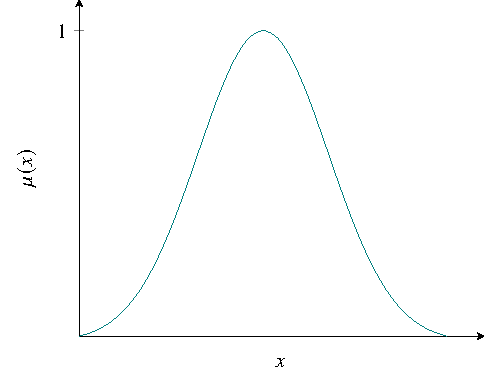
\includegraphics[width=.8\linewidth]{convex-fuzzy}
  \caption{Convex fuzzy set}
  \label{fig:sub-first}
\end{subfigure}
\begin{subfigure}{.4\textwidth}
  \centering
  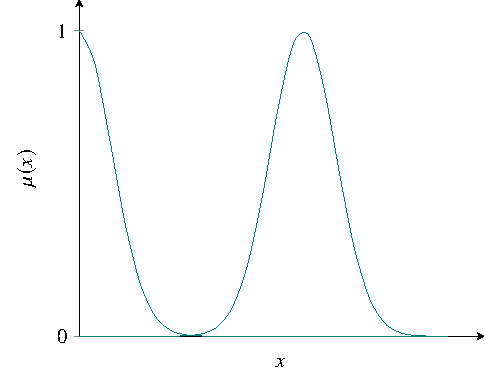
\includegraphics[width=.8\linewidth]{nonconvex-fuzzy}
  \caption{Non-convex fuzzy set}
  \label{fig:sub-second}
\end{subfigure}
\caption{Representation of membership functions of convex and non-convex fuzzy sets.}
\label{fig:convex-fuzzy}
\end{figure}


%--------------------------------------
%   Set-Theoretic Operations
%--------------------------------------

\subsection{Set-theoretic operations}

Most set-theoretic operations in the classical theory translate to fuzzy set theory in a natural way. We present a list of some of the most basic of these operations and their reinterpreted definitions in our setting, while introducing some of the notation that will be used in what follows.

\begin{definition}[Subset] If $A$ and $B$ are fuzzy sets, we say that $A$ is a subset of $B$, and we write $A \subseteq B$, if $\mu_A(x) \le \mu_B(x)$ for all $x \in X$.
\end{definition}

\begin{definition}[Union] The union of two fuzzy sets $A$ and $B$ is a fuzzy set $C = A \cup B$, whose MF is $\mu_C(x) = \max \, \{\mu_A(x), \mu_B(x) \} = \mu_A(x) \lmax \mu_B(x)$.
Alternatively, we can say that $C$ is the ``smallest'' fuzzy set that contains both $A$ and $B$.
\end{definition}

\begin{definition}[Intersection]
The intersection of two fuzzy sets $A$ and $B$ is a fuzzy set $C = A \cap B$, whose MF is $\mu_C(x) = \min \, \{\mu_A(x), \mu_B(x) \} = \mu_A(x) \lmin \mu_B(x)$.
As in the case of the union, $C$ can be viewed as the ``largest'' fuzzy set contained in both $A$ and $B$.
\end{definition}

\begin{definition}[Complement] The complement of a fuzzy set $A$, denoted by $\bar A$, is another fuzzy set defined by $\mu_{\bar A}(x) = 1- \mu_A(x)$.

\end{definition}

\begin{definition}[Cartesian product and co-product]
Let $A$ and $B$ be fuzzy sets in $X$ and $Y$, respectively. The \textit{Cartesian product} $A \times B$ is a fuzzy set in $X \times Y$ given by
\[
\mu_{A \times B}(x,y) = \mu_A(x) \lmin \mu_B(y).
\]
Similarly, the \textit{Cartesian co-product} $A+B$ is a fuzzy set in $X \times Y$ which has the membership function
\[
\mu_{A + B}(x,y) = \mu_A(x) \lmax \mu_B(y).
\]

\end{definition}

As it turns out, there are various ways of defining these basic operations in a fuzzy context, so we will refer to the operators used above as the \textit{classical} or \textit{standard fuzzy operators}. Other operators are discussed briefly in Subsection \ref{ssec:tnorm}. The choice of a specific fuzzy operator will depend on the specific problem we try to model, since different operators will most likely yield different outcomes and conclusions.

As with any new mathematical structure, one of the first steps after studying its basic properties is to study which operations preserve this structure, and how to generate new entities from existing ones. Regardless of the concrete operators employed, the operations just described provide us with the ability of generating new fuzzy sets from existing ones, while maintaining a reasonable interpretation of what they represent. Some of them will even preserve interesting properties of fuzzy sets, as seen in next result, whose proof can be derived by merely writing down the definitions of the concepts involved.

\begin{prop} An arbitrary intersection of convex fuzzy sets is a convex fuzzy set.
\end{prop}

Continuing along the same lines, we arrive at an important theorem regarding the creation of new fuzzy sets, stated by Zadeh himself. In short, it says that we can generate a fuzzy set that represents any structure, concept or relation that can be described with a (classical) mapping. A detailed introduction to this result and some insight as to its usefulness is given by E. Kerre in \cite{kerre2011tribute}.

\begin{theorem}[Extension principle] Let $f$ be a mapping from an $n$-dimensional product space $X_1 \times \dots \times X_n$ to a one-dimensional universe $Y$, and suppose $A_1, \dots, A_n$ are $n$ fuzzy sets in $X_1, \dots, X_n$, respectively. Then $f$ induces a fuzzy set $B$ in $Y$ defined by
\[
\mu_B(y) = \left\{ \begin{array}{cc}
	\sup\limits_{(x_1, \dots, x_n) = f^{-1}(y)} \, \min\limits_i \, \{ \mu_{A_i}(x_i) \}, & \text{if } f^{-1}(y) \ne \emptyset, \\
	0, & \text{if } f^{-1}(y) = \emptyset.
\end{array}\right.
\]

\end{theorem}

\begin{corollary} Let $f:X \to Y$ be a one-to-one mapping between one-dimensional spaces, and let $\mu_A$ represent a fuzzy set in $X$. Then, a fuzzy set $\tilde{f}(A)$ is induced in $Y$, given by
\[
\tilde{f}(A) = \int_X \mu_A(x) \slash f(x).
\]

\end{corollary}

\begin{example} Let $+:\R^2 \to \R$ represent the usual addition operation. Using the extension principle we can define the sum of two fuzzy sets $A$ and $B$ in $\R$ as a new fuzzy set $A+B$ with membership function given by
\[
\mu_{A+B}(z) = \sup \, \{\mu_A(x) \land \mu_B(y) \ | \ z = x + y \}, \quad \forall z \in \R.
\]

\end{example}

To conclude this brief exposition of operations between fuzzy sets, we now consider the general setting in which we have a multidimensional universe (i.e, a product space). In this case, it can be useful to think of fuzzy sets as a \textit{relation} among tuples of elements, each of which has a membership grade to the implied fuzzy set.

\begin{definition}[Fuzzy relation] Let $X$ and $Y$ be two universes of discourse. Then the fuzzy set
\[
\mathcal R = \{ ((x,y), \, \mu_\mathcal R (x,y) ) \ | \ (x,y) \in X \times Y \}
\]
represents a \textit{binary fuzzy relation} in $X \times Y$. A generalization to $n$-ary relations is straightforward.

\end{definition}

If $X$ and $Y$ are both discrete, we can express a fuzzy relation as a relation matrix $\mathcal R = (r_{ij})$, where $r_{ij}$ is the membership grade between the $ith$ element of $X$ and the $jth$ element of $Y$. As with fuzzy sets, we can operate with relations to produce new fuzzy sets, again using the classical operators previously described.

\begin{definition}[Max-min composition] \label{def:maxmin} Let $\mathcal{R}_1$ and $\mathcal{R}_2$ be two fuzzy relations defined on $X \times Y$ and $Y \times Z$, respectively. The max-min composition of $\mathcal R_1$ and $\mathcal R_2$ is a fuzzy set $\mathcal R_1 \circ \mathcal R_2$ in $X \times Z$ defined by
\[
\mu_{\mathcal R_1 \circ \mathcal R_2}(x,z) = \max_{y} \, \{ \mu_{\mathcal R_1}(x,y) \land \mu_{\mathcal R_2}(y,z) \}.
\]

\end{definition}

\begin{remark} If $\mathcal R_1$ and $\mathcal R_2$ are relation matrices, the calculation of $\mathcal R_1 \circ \mathcal R_2$ is almost the same as matrix multiplication, except that $\times$ and $+$ are replaced by $\land$ and $\lor$, respectively.

\end{remark}

\begin{prop} Let $\mathcal R, \mathcal S$ and $\mathcal T$ be binary relations on $X \times Y$, $Y \times Z$ and $Z \times W$, respectively, and let $\circ$ denote the max-min composition. Then, the following properties hold:

\begin{enumerate}
\item (Associativity) \ $\mathcal R \circ (\mathcal S \circ \mathcal T) = (\mathcal R \circ \mathcal S) \circ \mathcal T$.
\item (Distributivity  over union) \ $\mathcal R \circ (\mathcal S \cup \mathcal T) = (\mathcal R \circ \mathcal S) \cup (\mathcal R \circ \mathcal T)$.
\item (Weak distributivity over intersection) \ $\mathcal R \circ (\mathcal S \cap \mathcal T) \subseteq (\mathcal R \circ \mathcal S) \cap (\mathcal R \circ \mathcal T)$.
\item (Monotonicity) \ $\mathcal S \subseteq \mathcal T \implies \mathcal R \circ \mathcal S \subseteq \mathcal R \circ \mathcal T$.
\end{enumerate}

\end{prop}

\begin{proof}
  All four properties are easy to verify and follow directly from the well-known properties of the operators $\land$ and $\lor$.
\end{proof}

As one could expect, there are many possible definitions for a composition operator. For instance, another type of composition used in the literature (see \cite{markovsii2004solution, loetamonphong2001optimization}) is the \textit{max-product composition}.

\begin{definition}[Max-product composition] Assuming the same notation as above, the max-product composition is defined as follows:
\[
\mu_{\mathcal R_1 \circ \mathcal R_2}(x,z) = \max_{y} \, \{ \mu_{\mathcal R_1}(x,y) \mu_{\mathcal R_2}(y,z) \}.
\]

\end{definition}

%--------------------------------------
%   One-dimensional MFs
%--------------------------------------

\subsection{Parametrized one-dimensional MFs}

In this section, we describe the classes of parametrized functions commonly used to define one-dimensional fuzzy sets.

\begin{definition}[Triangular MF] Three parameters determine the $x$-coordinates of the three corners of a triangle:
\[
\operatorname{triangle}(x;a,b,c) = \max \left\{ \min \left\{ \frac{x-a}{b-a},\frac{c-x}{c-b}  \right\}, 0\right\}.
\]

\end{definition}

\begin{definition}[Trapezoidal MF] Four parameters determine the $x$-coordinates of the four corners of a trapezoid:
\[
\operatorname{trapezoid}(x;a,b,c,d) = \max \left\{ \min \left\{ \frac{x-a}{b-a},1, \frac{d-x}{d-c}  \right\}, 0\right\}.
\]

\end{definition}

\begin{definition}[Gaussian MF] It is determined by its center ($c$) and its width ($\sigma$) as follows:
\[
\operatorname{gaussian}(x;c,\sigma) = \exp \left(-\frac{1}{2}\left( \frac{x-c}{\sigma} \right)^2\right).
\]

\end{definition}

\begin{definition}[Generalized bell MF] It is specified by three parameters:
\[
\operatorname{bell}(x;a,b,c) = \frac{1}{1 + \left| \frac{x-c}{a}\right|^{2b}},
\]
where $b$ is usually positive.

\end{definition}

\begin{definition}[Sigmoidal MF] A sigmoidal MF is defined by
\[
\operatorname{sig}(x;a,c) = \frac{1}{1 + e^{-a(x-c)}},
\]
where $a$ controls the slope at the crossover point $x=c$.

\end{definition}

\begin{remark} Depending on the sign of the parameter $a$, a sigmoidal MF is inherently open right or left, and thus asymmetric. Closed and asymmetric MFs can be synthesized using either the absolute difference or the product of two sigmoidal functions.

\end{remark}

Triangular and trapezoidal membership functions are used because of their simplicity, both computational and interpretative. Nonetheless, they are composed of line segments and thus are not differentiable. This is where smooth MFs such as the Gaussian MF come into play, proving their usefulness in certain scenarios such as neuro-fuzzy systems. Some of these membership functions are shown in Figure \ref{fig:mfs}.


\begin{figure}[h!]
    \centering
    \begin{subfigure}[b]{0.4\textwidth}
        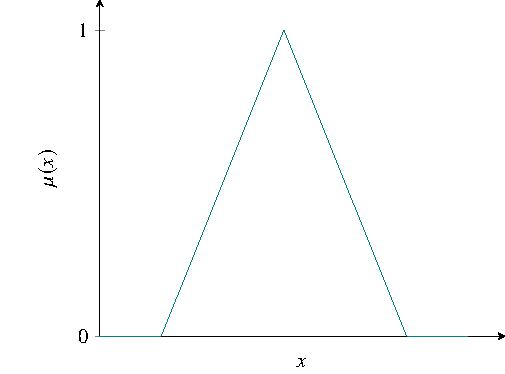
\includegraphics[width=\textwidth]{mf-triangle}
        \caption{Triangular MF}
    \end{subfigure}
    \begin{subfigure}[b]{0.4\textwidth}
        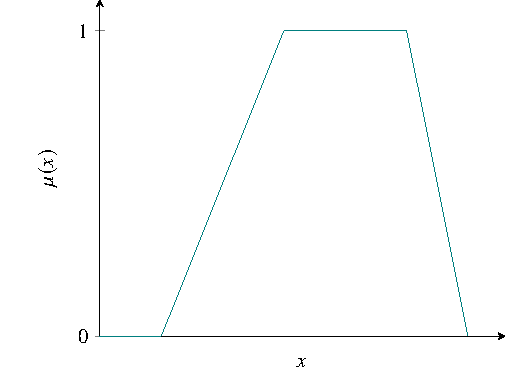
\includegraphics[width=\textwidth]{mf-trapezoid}
        \caption{Trapezoidal MF}
    \end{subfigure}
    %
    \begin{subfigure}[b]{0.4\textwidth}
        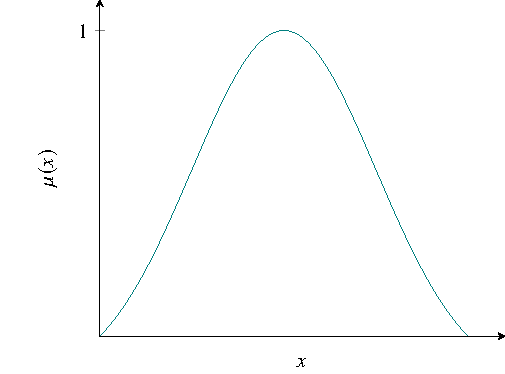
\includegraphics[width=\textwidth]{mf-gauss}
        \caption{Gaussian MF}
    \end{subfigure}
    \begin{subfigure}[b]{0.4\textwidth}
        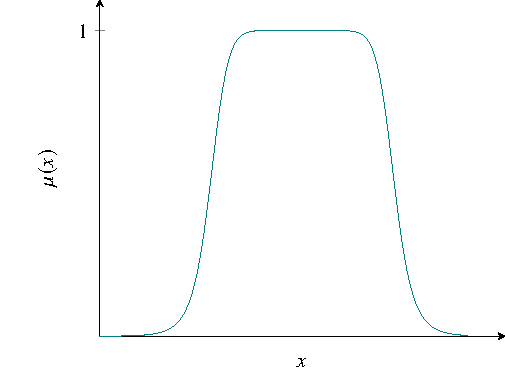
\includegraphics[width=\textwidth]{mf-bell}
        \caption{Generalized bell MF}
    \end{subfigure}
    \begin{subfigure}[b]{0.4\textwidth}
        \vspace{.5em}
        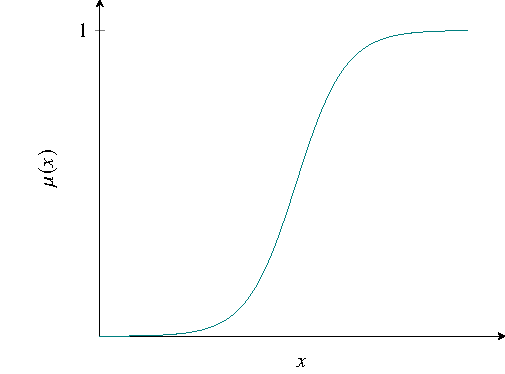
\includegraphics[width=\textwidth]{mf-sigmoid}
        \caption{Sigmoidal MF}
    \end{subfigure}
    \caption{Examples of different membership functions.}
    \label{fig:mfs}
\end{figure}

%--------------------------------------
%  Two-dimensional MFs
%--------------------------------------

\subsection{Two-dimensional MFs}

While it is possible to define membership functions in two or more dimensions, it is often desirable to begin in one dimension and build from there, effectively \textit{extending} the one-dimensional MFs defined above (or any other).

\begin{definition}[Cylindrical extension] If $A$ is a fuzzy set in $X$ and $Y$ is another universe, then the cylindrical extension of $A$ in $X \times Y$ is defined by
\[
c(A) = \int_{X\times Y} \mu_A(x) \slash (x,y).
\]

\end{definition}

We can also perform the inverse operation, that is, decompose a two-dimensional MF in two one-dimensional MFs.

\begin{definition}[Projections] Let $R$ be a two-dimensional fuzzy set on $X\times Y$. Then the projections of $R$ onto $X$ and $Y$ are defined as
\[
R_X = \int_X \max_y \, \mu_R(x,y) \slash x, \quad R_Y = \int_Y \max_x \, \mu_R(x,y) \slash y.
\]

\end{definition}

\begin{definition}[Composite MF] A two-dimensional MF is said to be \textit{composite} if it can be decomposed as an analytic expression of two MFs of one dimension; otherwise it is \textit{non-composite}.

\end{definition}

The Gaussian MF is arguably the most notable example of a composite MF, since it is a well known result that every $n$-dimensional Gaussian function is the product of $n$ one-dimensional Gaussian functions, scaled by some constant factor.


%----------------------------------------
%  Fuzzy Complemnt, T-norm and T-conorm
%----------------------------------------

\subsection{Fuzzy complement, T-norm and T-conorm} \label{ssec:tnorm}

Lastly, we explore the generalization of the classical fuzzy operators that have been described throughout this section.

\begin{definition}[Complement operator] A fuzzy complement operator is a continuous function $N:[0,1] \to [0,1]$ which meets the following axiomatic requirements:

\begin{enumerate}
	\item \textit{(Boundary)} \ $N(0)=1$ and $N(1)=0$.
	\item \textit{(Monotonicity)} \ $N(a) \ge N(b)$ if $a \le b$.
	\item \textit{(Involution)} \ $N(N(a)) = a$.
\end{enumerate}

\end{definition}

\begin{remark} Sometimes an operator verifying only $(i)$ and $(ii)$ is considered a fuzzy complement operator.

\end{remark}

\begin{example} One can routinely verify that the following two operators are fuzzy complement operators.
\begin{enumerate}
  \item \textit{(Sugeno's complement} \cite{sugeno1993fuzzy}$)$ $\displaystyle N_s(a) = \frac{1-a}{1+sa}$, where $s > -1$.
  \vspace{.25em}
  \item \textit{(Yager's complement} \cite{yager1979measure}$)$ $N_w(a) = (1-a^w)^{1/w}$, where $w>0$.
\end{enumerate}

\end{example}

\begin{definition}[$T$-norm operator] The intersection of two fuzzy sets $A$ and $B$ is specified in general by a function $T:[0,1]\times [0,1] \to [0,1]$, referred to as a $T$-norm operator, which aggregates two membership grades,
\[
\mu_{A \cap B}(x) = T(\mu_A(x), \mu_B(x)),
\]
and verifies several basic properties, namely:
\begin{enumerate}
	\item \textit{(Boundary)} \ $T(0,0) = 0$ and $T(a,1) = a$.
	\item \textit{(Monotonicity)} \ $T(a,b) \le T(c,d)$ if $a \le c$ and $b \le d$.
	\item \textit{(Commutativity)} \ $T(a,b) = T(b,a)$.
	\item \textit{(Associativity)} \ $T(a, T(b,c)) = T(T(a,b),c)$.
\end{enumerate}

\end{definition}

For the sake of completeness, here are four of the most frequently used $T$-norm operators:

\begin{enumerate}
	\item \textit{Minimum:} $T_{min}(a,b) = a \land b$.
	\item \textit{Algebraic product:} $T_{ap}(a,b)=ab$.
	\item \textit{Bounded product:} $T_{bp}(a,b) = 0 \lor (a+b-1)$.
	\item \textit{Drastic product:} $T_{dp}(a,b) = \begin{cases}
	                                      a, & \text{if } b = 1,\\
	                                      b, & \text{if } a = 1,\\
	                                      0, & \text{otherwise}.
                                          \end{cases}$
\end{enumerate}

\begin{definition}[$T$-conorm operator] Similarly, the union of two fuzzy sets $A$ and $B$ is specified in general by a function $S:[0,1]\times [0,1] \to [0,1]$, known as a $T$-conorm operator, which works in the same way as a $T$-norm, except that the boundary condition is now $S(1,1) = 1$ and $S(0,a) = a$.

\end{definition}

Corresponding to the four $T$-norm operators previously defined, we have the following $T$-conorm operators:

\begin{enumerate}
	\item \textit{Maximum:} $S_{max}(a,b) = a \lor b$.
	\item \textit{Algebraic sum:} $S_{as}(a,b)=a + b - ab$.
	\item \textit{Bounded sum:} $S_{bs}(a,b) = 1 \land (a+b)$.
	\item \textit{Drastic sum:} $S_{ds}(a,b) = \begin{cases}
	                                      a, & \text{if } b = 0,\\
	                                      b, & \text{if } a = 0,\\
	                                      1, & \text{otherwise}.
                                          \end{cases}$
\end{enumerate}

\begin{theorem}[Generalized De Morgan's Law] $T$-norms and $T$-conorms are duals which support the generalization of De Morgan's law:
\begin{align*}
	T(a,b) &= N(S(N(a),N(b))),\\
	S(a,b) &= N(T(N(a), N(b))).
\end{align*}

\end{theorem}

In fact, the eight operators showed above are dual in the sense of the generalized De Morgan's law.

\section{Fuzzy logic}

In this section we will study the methods and principles of \textit{fuzzy reasoning}, and present fuzzy logic as a multi-valued logic that generalizes the classical two-valued logic. If we think of the predicates \textit{true} and \textit{false} as being codified as $0$ and $1$, respectively, we can understand how to derive a \textit{fuzzy} logic theory in which every predicate has a \textit{truth grade} quantified by an appropriate membership function.

The whole new range of possible truth values gives something of a gray area in which propositions can fall. This is especially interesting in situations which involve a high degree of uncertainty, and thus its structure is difficult to capture with crisp values (if possible at all). The first example that comes to mind is what is known as \textit{natural language processing}, or the modelling of human speech to be ultimately processed by a computer. It is precisely this example that inspires the definitions and concepts that will be presented next, and it can be viewed as the starting point of the subsequent theory.


%--------------------------------------
%  Linguistic Variables
%--------------------------------------

\subsection{Linguistic variables}

\begin{definition}[Linguistic Variable] A linguistic variable is a quintuple $(x, T(x), X, G, M)$, in which:

\begin{enumerate}
	\item The symbol $x$ represents the name of the variable.
	\item $T(x)$ is the \textit{term set} of $x$, that is, the set of its \textit{linguistic values}.
	\item $X$ is, as usual, the universe of discourse.
	\item $G$ is a \textit{syntactic rule} which generates the terms in $T(x)$.
	\item $M$ is a semantic rule which associates with each linguistic value $A$ its \textit{meaning} $M(A)$, which in turn is nothing more than a fuzzy set in $X$.
\end{enumerate}

\end{definition}

\begin{example}
To help clarify the preceding definition, consider the concept of \textit{age} interpreted as a linguistic variable. Then its term set $T(\text{\textit{age}})$ could be something like the following:
\begin{center}
$T(\text{\textit{age}}) = \left\{\rule{0cm}{1.3cm}\right.$\begin{tabular}{ll}
\textit{young, not young, very young, not very young,} $\dots$, \\
\textit{middle aged, not middle aged,} $\dots$, \\
\textit{old, not old, very old, more or less old, not very old,} $\dots$, \\
\textit{not very young and not very old,}$\dots$
\end{tabular}$\left.\rule{0cm}{1.3cm}\right\}$,
\end{center}
where each term in $T(\text{\textit{age}})$ is characterized by a fuzzy set in a universe $X=[0,100]$.
\end{example}

The syntactic rule refers to the way that linguistic values are generated. We can see that the term set of the previous example consists of several \textit{primary terms} (\textit{young, middle aged, old}) modified by the \textit{negation} (\textit{not}) and/or \textit{adverbs} (\textit{very, more or less, quite,} and so forth), and linked by \textit{connectives} such as \textit{and, or, either} and \textit{neither}.

We shall come up with a way of treating all these modifiers as operators that change the meaning of their operands in a specified, context-independent fashion.

\begin{definition}[Concentration and dilation] Let $A$ be a linguistic value characterized by a fuzzy set with membership function $\mu_A$. Then $A^k$ is interpreted as a modified version of the original linguistic value expressed as
\[
A^k = \int_X (\mu_A(x))^k \slash x.
\]
In particular, the operation of \textit{concentration} is defined as $\operatorname{CON}(A)=A^2$, while that of \textit{dilation} is expressed by $\operatorname{DIL}(A)=A^{0.5}$.

\end{definition}

Conventionally, we take $\operatorname{CON}(A)$ and $\operatorname{DIL}(A)$ to be the result of applying the modifiers \textit{very} and \textit{more or less}, respectively, to the linguistic term $A$. Following the definitions in the previous chapter, we can interpret the negation operator \textit{not} and the connectives \textit{and}, \textit{or} as follows:
\begin{align*}
	\operatorname{NOT}(A) &= \neg A = \int_X 1 - \mu_A(x) \slash x,\\
	A \operatorname{AND} B &= A \cap B = \int_X \mu_A(x) \land \mu_B(x) \slash x,\\
	A \operatorname{OR} B &= A \cup B = \int_X \mu_A(x) \lor \mu_B(x) \slash x.
\end{align*}

\begin{definition}[Contrast intensification] The operation of contrast intensification on a linguistic value $A$ is defined by
\[
\operatorname{INT}(A) = \left\{ \begin{array}{ll}
	2A^2, & \text{if }  0 \le \mu_A(x) \le 0.5,\\
	\neg 2(\neg A)^2, & \text{if }  0.5 \le \mu_A(x) \le 1.
\end{array}\right.
\]
This operator has the effect of reducing the fuzziness of a linguistic value. In the extreme case of repeated applications, the fuzzy set becomes a crisp set with boundaries at the crossover points.

\end{definition}

Lastly, when we define MFs of linguistic values in a term set, it is intuitively reasonable to have these MFs roughly satisfy the requirement of orthogonality, which is described next.

\begin{definition}[Orthogonality] A term set $T= \{t_1, \dots, t_n\}$ of a linguistic variable $x$ on the universe $X$ is \textit{orthogonal} if it fulfills the following property:
\[
\sum_{i=1}^n \mu_{t_i}(x) = 1, \quad \forall x \in X,
\]
where each $t_i$ is a convex and normal fuzzy set defined on $X$.
\end{definition}


%--------------------------------------
%  Fuzzy If-Then Rules
%--------------------------------------

\subsection{Fuzzy if-then rules}

The core idea behind fuzzy reasoning is that the classical if-then rules of inference used in many systems can be reinterpreted under a fuzzy perspective, taking advantage of all the properties and easiness of interpretation that come with it.

\begin{definition}[Fuzzy if-then rules] If $A$ and $B$ are linguistic values, a fuzzy if-then rule associated with them assumes the form
\begin{center}
  if $x$ is $A$ then $y$ is $B$,
\end{center}
where ``$x$ is $A$'' is the \textit{antecedent} part and ``$y$ is $B$'' is the \textit{consequent} part. Sometimes we will abbreviate such a rule as $A\to B$.
\end{definition}

Some examples of fuzzy rules include \textit{if the patient's temperature is high, give them a moderate dose of medicine}, or \textit{tall people will get a big discount}. These rules are most useful, as we have already pointed out, when the concepts we are trying to model are difficult to describe in exact terms: is there a universally accepted height from which a person is considered to be tall? Is a body temperature of 38\textdegree{} indicative of a problem but $37.9$\textdegree{} is not?

Since a fuzzy if-then rule models a relation between two variables $x$ and $y$, it makes sense to interpret $A\to B$ as a fuzzy relation $\mathcal R$ given by a membership function $\mu_{\mathcal R} = f(\mu_A(x), \mu_B(y))$, for an appropriate choice of an implication function $f$ (usually a $T$-norm operator). Now we derive the basic operation of fuzzy reasoning, which consists of an \textit{approximate modus ponens}. Starting from the fuzzy rule \textit{if $x$ is $A$ then $y$ is $B$}, if we have the premise $x$ is $A'$, where $A'$ means an approximation of $A$, we can conclude that $y$ is $B'$, with $B'$ being an approximation of $B$. In other words, if $x$ is $A$ \textit{to a certain degree}, then $y$ is $B$ \textit{to a certain (possibly different) degree}. We give a precise meaning and structure to this process in the following definition.

\begin{definition}[Fuzzy reasoning] Let $X,Y$ be two universes of discourse and let $A, A'$ and $B$ be fuzzy sets in $X$, $X$ and $Y$, respectively. If $A\to B$ is a fuzzy implication, then a fuzzy set $B'$ is induced on $Y$, defined by
\[
B' = A' \circ (A \to B),
\]
where $\circ$ is the max-min composition (see Definition \ref{def:maxmin}), or equivalently,
\[
\mu_{B'}(y) = \lor_x (\mu_{A'}(x) \ \land \mu_{A \to B}(x, y)).
\]

\end{definition}

It goes without saying that we can have as many fuzzy rules as we want, and our ultimate goal will be to aggregate all of them together and produce a coherent reasoning system. Even though we have only considered the simplest case with one antecedent and one consequent, we can treat rules with multiple antecedents using the cartesian product operator, and rules with multiple consequent as the union of many rules with just one consequent. For example, we can have the following line of reasoning:

	\begin{center}
	  $x$ is $A'$ and $t$ is $B'$\\
    if $x$ is $A_1$ and $t$ is $B_1$ then $z$ is $C_1$\\
    if $x$ is $A_2$ and $t$ is $B_2$ then $z$ is $C_2$\\
    \rule{7cm}{0.4pt}\\
    $z$ is $C'$
  \end{center}
In this case, we interpret the first rule as a relation $\mathcal R_1 = A_1 \times B_1 \to C_1$ and the second one as $\mathcal R_2 = A_2 \times B_2 \to C_2$. Then, the induced fuzzy set $C'$ is given by
\[
C' = (A' \times B') \circ (\mathcal R_1 \circ \mathcal R_2) = C_1' \cup C_2',
\]
where $C_1'$ and $C_2'$ are the fuzzy sets inferred from the first and second rule, respectively.

\section{Fuzzy inference systems}

Now that we have gone over all the key elements in the theory of fuzzy reasoning, we are prepared to understand what a \textit{fuzzy inference system} (\acrshort{fis}) is. In summary, it is a system that maps an input space to an output space, using fuzzy techniques along the way as the main reasoning mechanism. Generally speaking it is made of four clearly differentiated parts:

\begin{enumerate}[1.]
  \item A \textit{fuzzification module}, which converts crisp inputs into fuzzy sets, with some predefined membership functions.
  \item A \textit{rule base} that contains a set of fuzzy if-then rules.
  \item An \textit{inference engine} that takes some input and employs the rules in the rule base to infer the corresponding output, using the fuzzy reasoning scheme described in the previous section. The membership functions in the output space are also predefined.
  \item A \textit{defuzzifying method} used to convert the output back to a crisp value, if necessary.
\end{enumerate}

A positive quality of a FIS is that its rule base can be easily modified with the addition of new rules or the adjustment of existing ones. The rules in the rule base can be defined by an expert based on their knowledge of the specific problem we are tackling, but they can also be \textit{learned from data}. This fact opens the door to the treatment of fuzzy systems with the techniques and learning algorithms that have been emerging over the course of the last decades in this field. This is precisely what we pursue: to build a fuzzy system that can learn and benefit from enormous amounts of data. This process will be discussed in depth in Chapter \ref{ch:implementation}.

One of the most important thing to take into account is that the choice of membership function is subjective, but not arbitrary. It heavily depends on the problem we are trying to solve, and selecting the appropriate MF for a given task usually gives much better results than choosing one either at random or one that gave good results on some entirely different problem.

Even though we have described every step of the inferring process in this and the previous sections, we summarize them below for completeness.

\begin{enumerate}[1.]
  \item In the first place, inputs to the system are \textit{fuzzified} and the membership grade of each input to the predefined fuzzy sets are calculated.
  \item Then, the \textit{firing strength} of each rule is computed, which usually consists on performing the fuzzy AND operation between the antecedents.
  \item Now the firing strength of each rule is combined with the consequent part to form an overall degree of satisfaction of the rule, known as the \textit{qualified consequent}. This is done as we described when we talked about implication operators, which in turn are commonly implemented with $T$-norm operators (e.g. the $\land$ operator).
  \item We aggregate all qualified consequents and choose the one that best represents the input value, for which the OR operator is the standard choice.
  \item Finally, we employ the aggregated output MF to obtain a crisp value as the output, i.e. a defuzzified value.
\end{enumerate}
Because of the use of fuzzy rules in the reasoning process, these systems are often called Fuzzy Rule-Based Systems (\acrshort{frbs}).
\subsection{Fuzzy system types}

To bring this exposition about fuzzy theory to an end, we present the two most common types of fuzzy systems used in practical applications. These two systems differ mainly in how they treat the output values.

\begin{definition}[Mamdani fuzzy inference system] A Mamdani fuzzy inference system (see \cite{madmani1975experiment}) is a FIS that takes an input $X=(X_1,\dots,X_n)$ and produces an output $Y = D(Y_1, \dots, Y_m)$, using rules of the form
\begin{center}
  if $X_1$ is $A_1$ and $X_2$ is $A_2$ and $\dots$ and $X_n$ is $A_n$\\
  then $Y_1$ is $B_1$ and $Y_2$ is $B_2$ and $\dots$ and $Y_m$ is $B_m$,
\end{center}
together with a defuzzification function $D:[0,1]^m \to \R^m$ to compute the final crisp values.
\end{definition}

The most common defuzzification method is the \textit{centroid of area} method, or \acrshort{coa} for short. It extracts a representative value from a fuzzy set, which can be thought of as the center of gravity of the area under its membership function. For a one-dimensional fuzzy set $A$ in a universe $Z$, it assumes the form
\[
z = \frac{\int_Z z\mu_A(z)\, dz}{\int_Z \mu_A(z)\, dz}.
\]
Other defuzzification methods are studied in the literature. A non-exhaustive classification of such methods can be found in \cite{leekwijck1999defuzzification}.

\begin{example}
  A typical single-input single-output Mamdani fuzzy model could be expressed as follows:
  \[
  \left\{ \begin{array}{l}
	\text{If $X$ is small then $Y$ is small}.\\
  \text{If $X$ is medium then $Y$ is large}.\\
	\text{If $X$ is large then $Y$ is very large}.
\end{array}\right.
\]
\end{example}

The other type of FIS that we will study is one in which the output is not a fuzzy set, but a crisp function of the input values. It is aimed at generating fuzzy rules from a given input-output data set, and is appropriate for solving regression problems.

\begin{definition}[TSK fuzzy inference system] A TSK fuzzy inference system (proposed by Takagi, Sugeno and Kang \cite{takagi1985identification, sugeno1988structure}) is a FIS that takes an input $X=(X_1,\dots,X_n)$ and produces an output $Y = (Y_1, \dots, Y_m)$, using rules of the form
\begin{center}
  if $X_1$ is $A_1$ and $X_2$ is $A_2$ and $\dots$ and $X_n$ is $A_n$\\
  then $Y_1$ is $f_1(X_1, \dots, X_n)$ and $Y_2$ is $f_2(X_1, \dots, X_n)$ and $\dots$ and $Y_m$ is $f_m(X_1, \dots, X_n)$,
\end{center}
where each $f_i$ is a crisp function of the input values (usually a polynomial).
\end{definition}

One thing to take into account is that the overall output is obtained via a \textit{weighted average} of the output of each rule (the weights being their firing strength), since now there are no fuzzy sets in the consequent part. This also eliminates the need for a defuzzification module, and thus improves the speed of the system.

\begin{example}
  A typical single-input TSK fuzzy model could be expressed as follows:
  \[
  \left\{ \begin{array}{l}
	\text{If $X$ is small then $Y=0.1X + 6$}.\\
  \text{If $X$ is medium then $Y=-0.5X -3$}.\\
	\text{If $X$ is large then $Y=X+2$}.
\end{array}\right.
\]
\end{example}


\chapter{Big Data}
%
% Copyright (c) 2020 Antonio Coín Castro
%
% This work is licensed under a
% Creative Commons Attribution-ShareAlike 4.0 International License.
%
% You should have received a copy of the license along with this
% work. If not, see <http://creativecommons.org/licenses/by-sa/4.0/>.

Since the beginning of time, we humans have always had the need to store information of some kind for a variety of applications: to keep track of the grain stock, to make a census of the population of a certain area, or simply to make a note for latter use. But it was not until the start of the so-called \textit{era of information} that the storage of data in a digital format became a reality and a part of everyday life. From then on, there has been an ever-increasing need for storage capacity, growing from kilobytes to megabytes to gigabytes and beyond in a mere few decades. But in recent years, the quantity of data that we collectively manage has grown so large that it is even hard to comprehend its scale. To put things into perspective, the total estimate of data ever created, captured or replicated amounts to 18 zettabytes (more than $10^{13}$ gigabytes) \cite{rydning2018digitization}. That is indeed \textit{a lot} of data.

Given the enormous quantity of information that we are constantly generating, it should not come as a surprise that the conventional ways of storing, manipulating and analyzing this information fail to accomplish their goal: they have become outdated. This is why the search for new approaches to this problem has recently gained traction in industry as well as in academia; we require new architectures and methods for dealing with such a big volume of data. It is precisely for this reason that the term \textit{Big Data} was coined. It refers to the manipulation and the extracting of information from data sets so large that they exceed the capabilities of most modern operating systems and hardware, and can't be handled with the usual data-processing methods within a reasonable elapsed time.

\section{Fundamental characteristics of Big Data}

First of all we need to clarify what we understand by Big Data. While the precise definition varies somewhat in the literature (see \cite{kitchin2016big} for example), there are a series of characteristics that any Big Data environment (problem, data set, etc.) should present in order for it to be considered as such. Coupled with these characteristics there are certain considerations to take into account, either as a direct result or as a side effect of working with large amounts of data. We explore all of these elements over the next subsections.

It should be noted that we will not consider a Big Data question the act of merely storing information with no other purpose than to preserve it. There should always be a particular problem (in the broad sense of the term) that is being solved by means of the data.

\subsection{The five V's}

The concept of the various \textit{V's of Big Data} has become a popular way of summarizing the principal characteristics that are desirable in a Big Data context. While the exact number and definition of these traits varies from author to author, they all share the same underlying principle: to capture the essence of what makes Big Data \textit{big}. We list below the ones that are deemed the most important, in no particular order.

\begin{enumerate}[1.]
  \item \textit{Volume}. It refers to the quantity of generated and stored data. It must be sufficient to draw meaningful conclusions and gain insight into the problem at hand. A necessary condition for establishing that some data has enough volume is that it exceeds the standard capacities of modern computers, which as of the year 2020 is in the terabytes.
  \item \textit{Velocity}. It relates to the speed or rate at which the data is generated or received. In some cases it includes real-time data processing, also known as \textit{streaming data}. In general, it is expected that the information be produced continually (think for example in a sensor of some kind).
  \item \textit{Variety}. The type and nature of the data also plays an important role. It includes both structured and unstructured data, drawn from various sources such as text, image, audio, etc.
  \item \textit{Veracity}. We can think of it as a way of measure how trustworthy the data is. The quality of the data can be affected by multiple factors such as inconsistencies, incompleteness or ambiguity, among others.
  \item \textit{Value}. It describes the added value that the collected data may have in the intended process, and the potential utility that can be extracted from the data. This value could change with time as the data is stored for a longer period, or even if the volume or velocity are modified.
\end{enumerate}


\subsection{Big Data algorithms}

Another relevant aspect apart from the above characteristics is \textit{how the data is being used}. In this work we focus on the analysis of said data to draw meaningul conclusions that could help solve a real-life problem. For this task the most common approach is to use the data to learn a specific pattern and try to generalize this behaviour to previously unseen data. This is essentially what is called a learning algorithm in the field of machine learning. These algorithms are designed to solve a \textit{learning problem}, which in turn is almost always categorized as a \textit{classification problem} or a \textit{regression problem}.
In general, a learning problem can be formally stated as follows:

\begin{quotation}
  \itshape \noindent
  Let $X$ be an input space and $Y$ an output space, and suppose there is some kind of unknown relation between them, modelled by a function $f:X\to Y$. Further suppose that there is an underlying probability distribution $\mathcal P$ on $X \times Y$. The problem consists on estimating $f$ using a set of $n$ samples $\mathcal D = \{ (x_i, f(x_i)) \ | \ i = 1,\dots,n \}$ drawn independently and identically distributed from $X \times Y$ according to $\mathcal P$.
\end{quotation}
If the output space is discrete we say it is a classification problem (the elements of $Y$ are regarded as labels), and if it consists on a continuous range of values, we say it is a regression problem. One common example is analyzing medical data to extract information about a certain disease, or trying to predict if a patient will develop a condition based on some previously collected data from sensors, tests, etc.

Although the problem of learning from data was not born along with Big Data, it certainly has to adapt to this new setting. Often the well-known algorithms to solve tasks involving a controlled amount of data cannot be directly implemented to solve Big Data problems, and have to be redesigned with an essential feature in mind: \textbf{scalability}. This property refers to the ability of algorithms to perform the task they were designed to do in a reasonable amount of time as the volume of data increases, if we equally increase the computation power of the machine where it is running. For example, an algorithm whose time complexity grows quadratically with the number of data points is not scalable, while one with a linear time complexity may very well be.

\subsection{Big Data ethics}

Since more and more data is being generated every day, there is a growing concern that this data could be used for malicious or unethical purposes. Of particular importance is the usage of \textit{personal data}, that is, data that could be used to identify a person or to extract information and patterns about their behaviour unbeknownst to them. In this regard there are a few principles that need to be taken into account when dealing with Big Data:

\begin{enumerate}[1.]
  \item \textit{Ownership}. This involves the rights over recorded data and the ability to exercise control over and limit the sharing of it. A recently passed European law called General Data Protection Regulation, or GDPR \cite{eu2016gdpr}, indicates that individuals own their personal data, and have a say in how it is being treated. The law clearly states that \textit{<<the processing of personal data should be designed to serve mankind>>}.
  \item \textit{Transaction transparency}. It refers to the right of any individual to have complete knowledge of why their data is being collected, how it is going to be used and for how long it will be stored, as well as how to ammend any part of the collected data.
  \item \textit{Consent}. Before any use of personal data there must be an informed, explicit and unambiguous consent from the subject of the information.
  \item \textit{Privacy}. The idea that a reasonable effort should be made to preseve the privacy of the subjects of the data being collected is an important one. Anonimity should be guaranteed and under no circumstances should the data be used to or facilitate the task of identifying a particular person without their explicit consent and knowledge.
  \item \textit{Openness}. In an ideal setting, all data should be freely available and open to the general public. This is especially important when it comes to data gathered by governments, both for transparency and accountability reasons.
\end{enumerate}

\section{Big Data architectures}

Having reviewed the main properties and characteristics of Big Data, we conclude this introduction presenting the principal architectures and methods for the treatment of this data. There are roughly three areas in which the process can be divided: storage, processing and analysis.

We have already covered the analysis step, which consists on applying suitable algorithms to try to extract meaningful conclusiones about the data, remembering that these algorithms must be developed in a scalable way. Not only should they be designed for scalability, but also adapted to be run on parallel architectures that allow the scalability to be implemented. In other words, in a Big Data environment it is typical to work with distributed machines, or \textit{clusters} of computers, so that more and more computing power can be easily added to the mix if needed.

Motivated by this approach arises the need for a method of storing data in multiple places in an efficient and safe way. Although there are multiple proposals to tackle this issue, one of the most prominent architectures is the \textit{Hadoop Distributed File System}\footnote{Hadoop was named after a toy elephant that belonged to the son of Doug Cutting, one of the main developers.}, or HDFS \cite{chansler2010hdfs}. It provides an interface to store and access data in a distributed file system, and it is designed to be fault-tolerant and reliable.

As for the processing of the data, the reference framework is the MapReduce programming model, proposed by Google in 2004 \cite{dean2004mapreduce}. It consists on a \textit{mapping} stage, in which transformations are performed on the data, and a \textit{reduce} stage that serves as a summarizing or aggregating operation. These tasks are handled in a parallel fashion, and all communications and data transfers are managed by the framework.

As a final comment, we should point out that a trend that has emerged to facilitate dealing with these architectures is \textit{cloud computing}. Companies are offering their hardware resources for the public to rent and use as a way of working with Big Data, eliminating the need of physically assembling and maintaining a cluster of machines.

\subsection{Apache Spark}
hadoop


\chapter{Design and implementation of fuzzy systems for Big Data}
\label{ch:fuzzy-bigdata}
%
% Copyright (c) 2020 Antonio Coín Castro
%
% This work is licensed under a
% Creative Commons Attribution-ShareAlike 4.0 International License.
%
% You should have received a copy of the license along with this
% work. If not, see <http://creativecommons.org/licenses/by-sa/4.0/>.

In this chapter we will concentrate on the design and implementation of several fuzzy systems for working with Big Data. While approaching these systems from a theoretical perspective as we have been doing throughout the text, we will shift our focus somewhat and also describe a number of implementations in an actual programming language. This part can be regarded as a more practical aspect of our work, a small software development project undertaken with the intent of fusing the ideas previously presented.

The language of choice is the Scala programming language, and the platform to develop our Big Data programs will be no other than Apache Spark. Although we will generally provide a high-level description of the algorithms, we will also insert occasional pieces of code that help clarify what we are trying to achieve, and even sometimes discuss technical aspects of the implementation or particularities of the language.

The interested reader can refer to \cite{suereth2012scala} or \cite{odersky2008programming} for a detailed introduction to Scala. Basic and intermediate notions of the interaction between Scala and Spark are also covered in \cite{karau2015learning}.

\section{Learning algorithms for fuzzy systems}

There are basically two different strategies to build FRBS, depending on the information available at the moment of its construction. The first way is to rely on human experts, inputting the knowledge manually into the system. This is one of the main tasks tackled in the field of \textit{knowledge engineering}, where knowledge engineers devise the best methods to extract and properly represent the knowledge from experts in the matter. The other way is to try to learn the rules and behaviour of the system from the data, by using several learning methods. We will concentrate on the latter approach.

Generally speaking, learning algorihms for FRBSs can be decomposed in two stages: a structure identification step and a parameter tuning phase. In the first one, the structure and size of the rulebase is estimated, while in the second one the parameters corresponding to the various membership functions involved are optimized. These steps can be performed sequentially or in a simultaneous way.

While these algorithms are tailored to work with fuzzy systems, the restrictions and particularities of the general learning algorithms still apply. That is, choosing a specific algorithm is only one step of the full learning process: data preprocessing, dimensionality reduction, parameter selection, etc. A number of software libraries have been developed to work with fuzzy systems, among which we would like to highlight the \verb|frbs| R package \cite{riza2015frbs}. It gathers a multitude of classification and regression algorithms under a common API that focuses on easiness of use.

Before we specify the algorithms implemented, we present an overview of the three main types of learning algorithms for FRBSs.

\subsection{Space partition algorithms}

These algorithms are designed so that a partition on the input and output spaces is established, and rules are derived from the grade in which each data point represents each of these partitions. In other words, rules are created \textit{ad-hoc} directly from the data.

The parameters of the membership functions are dependent on the specific technique used to partition the spaces, and the expressions used to measure the affinity of each point to each partition. A notable special case is the use of \textit{clustering algorithms} to make the partitions. In this case, each centroid acts as a fuzzy rule, with a membership function that measures the grade in which each points belongs to each centroid. This is known as \textit{fuzzy clustering}, and differs from classical clustering algorithms in that each point generally belongs to every cluster to a greater or lesser extent, not just to one of them.

\subsection{Neural network algorithms}

As their name indicates, these algorithms are based on the concept of artifical neural networks. These structures have been adapted from the field of machine learning and more precisely of deep learning, where they are widely used and serve as the basis of multiple state of the art algorithms (see for example \cite{lecun2015deep}).

The FRBS is usually generated beforehand, and it is then adapted to fit a neural network structure. This network is used as a way of tuning the parameters of the membership function using the backpropagation algorithm, and thus retaining all the advantages of this technique. A typical neuro-fuzzy system has a layer that represents the membership functions of the linguistic values associated with the input variables, an antecedent layer that represents the antecedent parts of every rule, a consequent layer to express the consequent of the rules, and a defuzzification layer to provide a final response. Commonly there are weights involved in the process that calibrate the importance of each rule, and they can also be adjusted when training the network.

\subsection{Genetic algorithms}

We arrive at the last type of FRBS considered here, which is based on genetic algorithms. Ample research has been conducted on this topic, and the reader can refer to \cite{cordon2011historical} for a historical review or to \cite{cordon2001genetic} for a whole book on the subject.

The philosophy behind these algorithms is similar to that of the neuro-fuzzy systems: an initial structure is established, and then a genetic method is adapted to tune a specified set of parameters. But genetic algorithms can also be used to generate the whole structure from the start, as shown in \cite{cordon2001generating}. As an alternative to neuro-fuzzy systems, these algorithms present all the advantages (as well as the disadvantages) of the standard genetic methods. Since we will not be developing any algorithm that falls in this category, we mention a couple of them that are studied in the literature.

\begin{enumerate}[1.]
  \item The first one is a basic genetic fuzzy system based on Thrift's method \cite{thrift1991genetic} of integer coding. In this method, each possible rule represents a chromosome, and a new population is obtained by applying the usual crossover and mutation operators (although mutations are adapted to this particular setting), and follows an elitist scheme. The fitness of an individual is calculated as the mean squared error between predictions and actual values, as outputed by the system.
  \item Cordón and Herrera proposed the D-MOGUL method \cite{cordon1997three} to automatically generate a complete knowledge base; it uses a genetic algorithm to determine the structure of the fuzzy rules and the parameters of the membership functions simultaneously. It consists on three steps:
  \begin{itemize}
    \item An iterative \textit{rule generation} process that explores the search space for rules that satisfy certain desirable conditions. A partition of the input space consisting on triangular membership functions is considered.
    \item A \textit{genetic simplification phase}, that eliminates redundant rules from the previous step by exploring the subsets of rules that best cooperate among themselves.
    \item A \textit{genetic tuning phase} in which membership parameters are adjusted to try to maximize the accuracy of the final model.
  \end{itemize}
\end{enumerate}

\section{Cost estimation and planning}

<Description of the planning of the project and the estimated costs of both human and hardware resources.>

\section{Clustering algorithms}
\subsection{Subtractive clustering}
\subsection{Fuzzy C-Means}
\section{Neuro-fuzzy algorithm: HYFIS}


\setpartpreamble[u][\textwidth]{\vspace*{2em}\centering \large \emph{Mathematics}}
\part{Ordinary differential equations not solved for the derivative}

\chapter{Introduction}
%
% Copyright (c) 2020 Antonio Coín Castro
%
% This work is licensed under a
% Creative Commons Attribution-ShareAlike 4.0 International License.
%
% You should have received a copy of the license along with this
% work. If not, see <http://creativecommons.org/licenses/by-sa/4.0/>.

<Detailed introduction to the work done, with objectives, motivation, etc.>


\chapter{Basic concepts}
%
% Copyright (c) 2020 Antonio Coín Castro
%
% This work is licensed under a
% Creative Commons Attribution-ShareAlike 4.0 International License.
%
% You should have received a copy of the license along with this
% work. If not, see <http://creativecommons.org/licenses/by-sa/4.0/>.

In this chapter we will introduce the basic terminology needed to understand the theory that will subsequently be developed. We will present ordinary differential equations and their solutions in a rigorous manner, as well as some concepts intimately related to them, such as integral curves and initial value problems, and analyze how these equations fit into the general theory of differentiable functions. At the same time, we will set the notation that will be used throughout the exposition. The main reference for this chapter is \cite{petrovski1966ordinary}.

\section{Ordinary differential equations}

By an \textit{ordinary differential equation of order $n$} we mean a relation of the form
\begin{equation}
\label{eq:ode}
F(x, y, y', \dots, y^{(n)}) = 0,
\end{equation}
where $F$ is a real-valued function of $n+1$ real variables, $x$ is an independent variable, $y=y(x)$ is an unknown function and $y', \dots, y^{(n)}$ are the first $n$ derivatives of this function with respect to $x$. When the value of $n$ is understood or simply not relevant, we will refer to \eqref{eq:ode} only as an ordinary differential equation (\acrshort{ode}), with the word \textit{ordinary} meaning that the unknown function depends solely on one independent variable. A central concept in our study will be that of a solution of such a differential equation, which is rigorously defined below.

\begin{definition}
  \label{def:solution}
  A \textit{solution} of the differential equation \eqref{eq:ode} is a function $\phi: I \to \R$, where $I=(a,b)$, $-\infty \leq a < b \leq \infty$ is some open interval of the real line, satisfying the following conditions:

  \begin{enumerate}
    \item The function $\phi$ has derivatives up to order $n$.
    \item The identity $F(x, \phi(x), \phi'(x), \dots, \phi^{(n)}(x)) = 0$ holds for all $x \in I$.
  \end{enumerate}
  The process of finding solutions of a differential equation is also known as \textit{integrating} the equation.
\end{definition}

From now on, unless otherwise stated we will restrict ourselves to \textit{first order} ODEs, which take the general form
\begin{equation}\label{eq:fode}
  F(x,y,y') = 0,
\end{equation}
and thus their solutions are differentiable functions of $x$ that reduce the equation to an identity when substituted for $y$. Furthermore, we will initially consider differential equations in \textit{explicit} form, that is,
\begin{equation}
  \label{eq:fode-explicit}
  y' = f(x, y),
\end{equation}
and we will assume that the function $f(x,y)$ is defined on some domain (open and connected subset) $G$ of the $(x,y)$-plane.

\begin{remark}
  Sometimes we will find it more useful to use Leibniz's notation and express the above equation as
  \begin{equation*}
    \der = f(x,y).
  \end{equation*}

\end{remark}

\section{Geometric interpretation of ODEs}

Continuing our description of differential equations, we shall now present a natural interpretation of equations such as \eqref{eq:fode-explicit} and a way to visualize them in the plane. To begin with, suppose that we draw a short line segment through every point $(x,y)$ of $G$ with slope equal to $f(x,y)$, obtaining a set of directions in $G$ that is called the \textit{direction field} of equation \eqref{eq:fode-explicit}. In other words, we transform our (known) function $f$ in a vector field on its domain. At this point we can restate the problem of solving \eqref{eq:fode-explicit} from a geometric perspective:
\begin{quotation}
  \itshape \noindent
  Find all differentiable curves $y=\phi(x)$ in $G$ whose tangents have directions belonging to the direction field of \eqref{eq:fode-explicit}.
\end{quotation}
To see how this is equivalent to solving \eqref{eq:fode-explicit}, one need only recall that the slope of the tangent of a (differentiable) curve at any point coincides with its derivative at that point, and then look at Definition \ref{def:solution}. However, this formulation of the problem has two noticeable caveats from a geometric point of view:

\begin{enumerate}[1.]
  \item By considering only \textit{graphs} over the $x$-axis we are excluding curves that are intersected more than once by vertical lines.
  \item The imposition that the slope of the direction field generated in $G$ be given by $f$ automatically excludes directions parallel to the $y$-axis, because $f$ would need to be infinite at those points.
\end{enumerate}

We are interested in looking at solutions of differential equations in a more general setting. This is why, based on the previous reformulation, we will develop a broader concept of solution with a strong geometrical meaning, one that will address both difficulties outlined above. In the first place, we allow general curves in parametric form, that is, $x=\lambda(t)$, $y=\mu(t)$, $-\infty \leq \alpha < t < \beta \leq \infty$. This solves the first problem. To overcome the second limitation, in addition to equation \eqref{eq:fode-explicit} we consider the associated differential equation
\begin{equation}
  \tag{\ref*{eq:fode-explicit}'}
  \label{eq:fode-explicit1}
  \frac{dx}{dy} = f_1(x,y),
\end{equation}
where
\begin{equation*}
  f_1(x,y) = \frac{1}{f(x,y)}.
\end{equation*}
The rationale behind this decision is to allow the function $f$ to become infinite at some points (representing a vertical slope), and shift our perspective from the $x$-axis to the $y$-axis at those points. In this way, at points where both $f$ and $f_1$ are defined we can use either \eqref{eq:fode-explicit} or \eqref{eq:fode-explicit1} to construct the direction field, but we use \eqref{eq:fode-explicit1} at points where $f$ becomes infinite\footnote{At each point of $G$, at least one of $f$ or $f_1$ is always defined, for $f=0$ if and only if $f_1$ is infinite, and $f_1=0$ if and only if $f$ is infinite.}.

We are now ready to define our new, more general concept of solution, which will necessarily be related not only to the original equation, but also to the newly defined associated equation. We will restrict ourselves to the class of \textit{smooth} \textit{regular} curves, that is, continuously differentiable curves with non-vanishing derivative everywhere. From now on, all curves will implicitly be assumed to belong to this class.

\begin{definition}\label{def:integral-curves}
  An \textit{integral curve} of equations \eqref{eq:fode-explicit} and \eqref{eq:fode-explicit1} is a smooth regular curve whose tangent at each point has a direction specified by the direction field of said equations.
\end{definition}

Given that equations \eqref{eq:fode-explicit} and \eqref{eq:fode-explicit1} are closely related, sometimes we will use the singular form to encompass both of them as a single equation. As we are looking at curves in parametric form, to obtain an explicit formula in this case we may first apply the chain rule,
\begin{equation*}
  \frac{dy}{dt} = \der \frac{dx}{dt},
\end{equation*}
and then we solve for $dy/dx$, getting
\begin{equation}
  \label{eq:fode-mn}
  \der = \frac{dy/dt}{dx/dt} = \frac{M(x, y)}{N(x, y)}.
\end{equation}
If the chosen curve does indeed satisfy the equation, then $f = M/N$ will hold. For simplicity we will seldom write down explicitly the associated equation,
\begin{equation}
  \tag{\ref*{eq:fode-mn}'}
  \frac{dx}{dy} = \frac{N(x,y)}{M(x,y)} = f_1(x,y),
\end{equation}
but we shall sometimes write \eqref{eq:fode-mn} as
\begin{equation*}
  M\,dx - N\, dy = 0,
\end{equation*}
to stress the symmetry in $x$ and $y$. This equation specifies a direction field at every point where both $M$ and $N$ are defined and at least one of them is nonzero.

Even though we are allowing general curves in parametric form, they are not (the graph of) a true solution of our equation unless we restrict them to some interval in which they can be expressed as a graph. We can think of the family of all solutions to equation \eqref{eq:fode-explicit} as a subset of the family of integral curves of \eqref{eq:fode-explicit} and \eqref{eq:fode-explicit1}, restricted to a suitable interval if need be. An example visualization of direction fields and integral curves is shown in Figure \ref{fig:integral-curves-ex}.

\begin{figure}[h!]
  \centering
  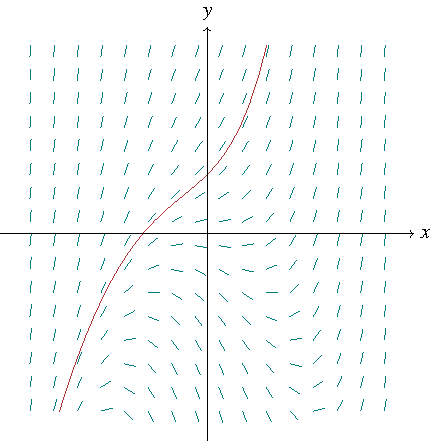
\includegraphics[width=.5\textwidth]{integral-curves-1}
  \caption{Direction field of the equation $y'=x^2+y$ near the origin and a particular integral curve.}
  \label{fig:integral-curves-ex}
\end{figure}

The requirement that integral curves be regular guarantees that we can always shrink their domain so that they become a graph, and hence a solution to our differential equation. The following result delves into that question.

\begin{prop}
  Every point in a smooth regular curve belongs to an arc which is a smooth graph.
\end{prop}

\begin{proof}
  Let $x=\lambda(t)$, $y=\mu(t)$, $\alpha < t < \beta$ be a smooth regular curve, and pick $t_0 \in (\alpha, \beta)$. The regularity of the curve guarantees that either $\lambda'(t_0)$ or $\mu'(t_0)$ is nonzero, so suppose without loss of generality that $\lambda'(t_0) \neq 0$. Since $\lambda'(t_0)$ is continuous by assumption, there exists an $\epsilon > 0$ such that $\lambda'(t)\neq 0$ for $t \in (t_0 - \epsilon, t_0 + \epsilon)$, and then the equation $x=\lambda(t)$ has a unique smooth solution in $t$ by virtue of the \textit{inverse function theorem} (see \cite[372]{apostol1974analysis}). Then, by eventually shrinking $\epsilon$ we may write $t=\psi(x)$, $\lambda(t_0 - \epsilon) < x < \lambda(t_0 + \epsilon)$. Substituting in $y=\mu(t)$ yields $y=\mu(\psi(x)) = \phi(x)$, $\lambda(t_0 - \epsilon) < x < \lambda(t_0 + \epsilon)$, which is the equation of a smooth graph.
\end{proof}

\begin{remark} The conditions on integral curves in Definition \ref{def:integral-curves} imply that our solutions are also smooth, that is, continuously differentiable.
\end{remark}

We can illustrate the previous definitions and properties with a simple example.

\begin{example}
  Consider the equation
  \begin{equation*}
    \der = \frac{y}{x},
  \end{equation*}
  which we can also write as
  \begin{equation*}
    x\,dy = y\,dx.
  \end{equation*}
  Solving it by elementary methods gives the family of solutions
  \begin{equation*}
    y =kx, \quad x \in \R - \{0\}, \ k \in \R.
  \end{equation*}
  On the other hand, this equation defines a direction field in the whole plane minus the origin. To find its integral curves we consider the associated equation $dx/dy = x/y$ in the subset
  \begin{equation*}
    \{(0, y): y \in \R - \{0\}\}
  \end{equation*}
  of the plane. Combining both equations we can see that the set of all integral curves is given by the relation
  \begin{equation*}
    ax+by=0, \quad (x,y), (a, b) \in \R^2 - \{(0,0)\}.
  \end{equation*}
  The direction field is shown schematically in Figure \ref{fig:integral-curves-ex-2}. Notice that we have found two integral curves for this equation that are not the graph of any solution, namely the two vertical rays emanating from the origin.
  \begin{figure}[h!]
    \centering
    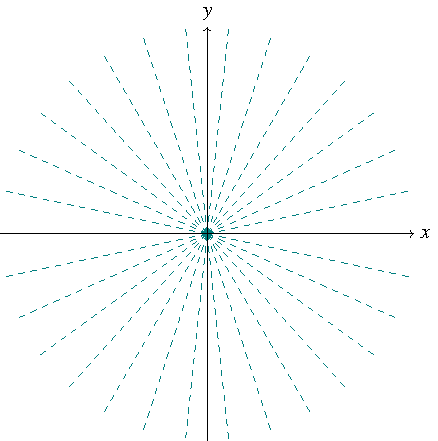
\includegraphics[width=.5\textwidth]{integral-curves-2}
    \caption{Direction field of the equation $x\,dy = y\, dx$ near the origin.}
    \label{fig:integral-curves-ex-2}
  \end{figure}
\end{example}

As a closing remark, we note that we could have ignored the directions parallel to the $y$-axis altogether, and we still would have ended up with a well defined, reasonable concept of integral curve. This is in fact what Arnold does in \cite{cooke1992ordinary}. However, taking these conflicting points into account will allow us to better study and understand \textit{singularities} of the function $f$, allowing for a more general perspective and broadening the scope of this work.

\section{Existence and uniqueness of solutions}

So far we have been talking about solutions of a differential equation without stopping to think even if such solutions exist in the first place. Could we come up with an equation which has no solutions at all? To answer this question, remember that any possible solution is assumed to be smooth, and thus its derivative verifies the \textit{intermediate value theorem}\footnote{\label{fn:darboux} A similar argument for non-smooth solutions may be given using \textit{Darboux's theorem} \cite[112]{apostol1974analysis}, which states that the derivative of any differentiable function that takes two different values on an interval must take every value in between.}. But this derivative must be equal to $f$, so it suffices to choose a function that does not have the intermediate value property. For example, if we consider the famous Dirichlet function
\begin{equation*}
  g(x) = \begin{cases}
    1  & \text{if } x \in \mathbb{Q},\\
    0  &\text{elsewhere},
\end{cases}
\end{equation*}
then the equation $y'=f(x, y) = g(x)$ has no solutions.

From this example we can speculate that the lack of continuity of $f(x,y)$ is the key property that makes the equation unsolvable. This is indeed the case, as it turns out that existence of solutions is always guaranteed if we impose that $f$ be continuous.

\begin{theorem}[Peano's existence theorem] Let $f(x,y)$ be a continuous function on a domain $G\subset \R^2$. Then the differential equation
  \begin{equation*}
    y' = f(x,y)
  \end{equation*}
has at least one solution in $G$. Moreover, if $f$ is continuous on a neighbourhood of a point $(x_0, y_0) \in G$, then there exists a solution $\phi$ defined on a neighbourhood of $x_0$ satisfying $\phi(x_0)=y_0$.
\end{theorem}

\begin{proof}
  See \cite{peano1890demonstration} for Peano's original 1890 proof, which uses a method known as successive approximations. Shorter proofs have been proposed since, many using topological arguments such as fixed points theorems (see for example \cite[14]{hale1980ode}).
\end{proof}

\begin{remark} If we assume continuity of the function $f$, then the smoothness of any solution comes as a consequence and not as a hypothesis, since $\phi'(x) = f(x, \phi(x))$. In fact, the level of regularity of the function $f$ translates in a similar manner to the solutions: if $f$ has continuous derivatives up to order $m$, then any solution to $y'=f(x,y)$ has continuous derivatives up to order $m+1$.

\end{remark}

The concept of a solution passing through a predefined point is not incidental to our study, but it plays a major role in much of the subsequent theory, which is why it merits its own denomination. A differential equation $y'=f(x,y)$ coupled with an \textit{initial condition} $y(x_0)=y_0$ is called an \textit{initial value problem}, often abbreviated as \acrshort{ivp}. With this new definition in mind, Peano's theorem states that every initial value problem defined by a continuous function has at least one solution, or more generally, that there is at least one integral curve of the equation passing through the selected point.

Together with the question of existence comes inevitably the issue of uniqueness. Peano's theorem guarantees that under mild conditions a solution to an initial value problem always exists, but it does not say anything about it being unique. It is not hard to think of an example in which uniqueness of solution is violated. For instance, it is immediate to verify that the IVP

\begin{equation*}
  \begin{cases} y' = 3y^{2/3},\\
    y(0)=0

  \end{cases}
\end{equation*}
has two valid solutions: $y=0$ and $y=x^3$. Thus some kind of additional condition is needed to ensure that one and only one integral curve passes through a given point, as the following theorem asserts.

\begin{theorem}[Picard-Lindelöf] \label{th:picard}
  Let $G \subset \R^2$ be a domain in the plane, and suppose $f:G \to \R$ is a continuous function that locally satisfies a Lipschitz condition in the second variable, that is, for every $p \in G$ there exists a neighbourhood $U_p$ of $p$ in $G$ and a constant $L>0$ such that
\begin{equation*}
  \abs{f(x, y_2) - f(x, y_1)} \leq L\abs{y_2 - y_1}
\end{equation*}
whenever $(x,y_1),(x,y_2) \in U_p$. Then for every point $(x_0, y_0) \in G$ the initial value problem
  \begin{equation}
  \begin{cases} y' = f(x, y) & \text{in } G,\\
    y(x_0)= y_0
  \end{cases}
\end{equation}
has exactly one solution.
\end{theorem}

\begin{proof}
  A proof in modern terms can be found in \cite[36]{teschl2012ordinary}. The idea is to construct a sequence of approximate solutions, the so-called method of \textit{Picard iterations}, and then leverage the Lipschitz condition to apply the \textit{contraction principle}\footnote{Also known as \textit{Banach fixed point theorem}, after Polish mathematician Stefan Banach who first proved it in 1922 \cite{banach1922operations}.}.
\end{proof}

\begin{remark}
  The Lipschitz condition on Theorem \ref{th:picard} can be relaxed to a condition on the partial derivative. The theorem remains true, via a direct application of the \textit{mean value theorem}, if $\partial f / \partial y$ is locally bounded, which in turn holds if said partial derivative is continuous on $G$. This condition is often easier to check.
\end{remark}

Bringing back the geometric interpretation of differential equations, it is straightforward to see that at points where there is uniqueness of solutions two integral curves can never be tangent to each other (they cannot cross either by definition). However, it is precisely the points in which uniqueness fails that interest us, and we will study them in depth in the following chapter.


\chapter{Implicit equations}
%
% Copyright (c) 2020 Antonio Coín Castro
%
% This work is licensed under a
% Creative Commons Attribution-ShareAlike 4.0 International License.
%
% You should have received a copy of the license along with this
% work. If not, see <http://creativecommons.org/licenses/by-sa/4.0/>.

Having presented ordinary differential equations and their solutions in the previous chapter, we now focus on our main goal: the study and understanding of \textit{implicit} differential equations, that is, equations which are not solved for the derivative $y'$. Since we cannot put this type of equations into explicit form, all the theory discussed earlier does not apply directly to this case, and thus we want to find a general framework that allows for the treatment of these equations from a theoretical point of view. For this task we will refer to \cite[\S \ 25]{petrovski1966ordinary} and \cite[\S \ 3]{arnold2012geometrical}.

Given that equations are expressed in the general or implicit form, it makes sense to think that the \textit{implicit function theorem} will play a significant role in disentangling the complexities behind this formulation of differential equations, and that it will tell us something about their local behaviour. In an effort to provide all the necessary tools for the study we are about to undertake, we write down the statement of this famous theorem below.

\begin{theorem}[Implicit function theorem]
Let $D$ be an open set in $\R^{n+m}$ with coordinates $(x, y)$ and let $F:D \to \R^m$ be continuously differentiable. If $(a,b)\in D$ verifies $F(a,b)=0$ and the Jacobian matrix $\frac{\partial F}{\partial y}(a, b)$ is nonsingular, then there exists an open set $U \subset \R^n$ with $a \in U$ and a unique $\mathcal C^1$ function $f:U\to \R^m$ such that:
\begin{enumerate}
  \item $f(a)=b$.
  \item $F(x, f(x)) = 0$ for all $x$ in $U$.
  \item The Jacobian matrix of $f$ is given by the matrix product
  \[
    Jf(x) = - \left( \frac{\partial F}{\partial y}(x, f(x))\right)^{-1} \left( \frac{\partial F}{\partial x}(x, f(x)) \right), \quad x \in U.
  \]
\end{enumerate}
\end{theorem}

\begin{proof}
A standard proof employing the equally renowned inverse function theorem can be found in \cite[374]{apostol1974analysis}. The last differentiation formula is obtained by differentiating the expression $F(x,f(x)) = 0$ and applying the chain rule.
\end{proof}

Even though we have stated the theorem for arbitrary dimensions, we will only apply it when $n=2$ and $m=1$, making the Jacobian matrix a single partial derivative. In fact, we recover the notation established in the previous chapter, and henceforth consider a function $F:\R^3 \to \R$ in $(x,y,p)$-space and the associated differential equation
\begin{equation}\label{eq:ode-implicit}
  F(x,y,y') = 0.
\end{equation}
Also, following a standard notation, we will denote by $F_x$, $F_y$ and $F_p$ the partial derivatives of the function $F$ with respect to each of its three variables $x$, $y$ and $p$. Then, the theorem assumes the following form:

\begin{corollary} \label{cor:implicit}
  Let $D$ be an open subset of $\R^3$ and let $F:D \to \R$ be continuously differentiable. If $(x_0, y_0, p_0) \in D$ verifies $F(x_0, y_0, p_0) = 0$ and $F_p(x_0,y_0,p_0) \neq 0$, then there exists an open set $U\subset \R^2$ containing $(x_0, y_0)$ and a unique $\mathcal C^1$ function $f:U\to \R$ such that $p_0=f(x_0,y_0)$ and $F(x, y, f(x,y))=0$ for all $(x, y) \in U$. Moreover, the partial derivative of $f$ with respect to its second variable is given by
  \begin{equation} \label{eq:der-formula}
  \frac{\partial f}{\partial y}(x, y) = - \frac{F_y(x,y, f(x,y))}{F_p(x, y, f(x,y))}.
\end{equation}
\end{corollary}

\section{Integral curves of implicit equations}

In this case we will start with an example. If we consider the differential equation
\begin{equation} \label{eq:ex1}
  (y')^2 = y,
\end{equation}
we should immediatly observe that this expression is an abbreviation for two distinct explicit differential equations: $y'=\sqrt y$ and $y'=-\sqrt y$, for $y > 0$. Each of these equations produces a direction field, as seen in Figure \ref{fig:ex1}, and each of them separately satisfies an existence and uniqueness theorem on its domain, though clearly the uniqueness of solution fails when combining them. Nevertheless, we would like to examine this kind of equations as a whole, and establish general conditions for their treatment.

\begin{figure}[h!]
\centering
\begin{subfigure}{.6\textwidth}
  \centering
  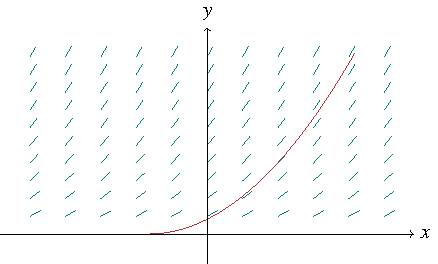
\includegraphics[width=\linewidth]{ex1}
\end{subfigure}
\begin{subfigure}{.6\textwidth}
  \centering
  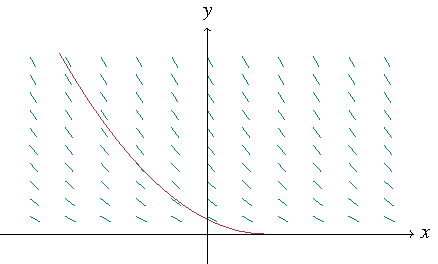
\includegraphics[width=\linewidth]{ex2}
\end{subfigure}
\caption{Direction fields of the two equations combined in the notation $(y')^2=y$.}
\label{fig:ex1}
\end{figure}

One thing to note from the beggining is that there are some occasions in which implicit equations can be put in explicit form, at least in theory. That is, there is a set of conditions that, when satisfied, guarantee that the equation is equivalent to another one in explicit form. Of course, in nontrivial cases this result will only hold locally, and as one would expect it is a direct consequence of the aforementioned implicit function theorem.

\begin{theorem} \label{th:implicit-basic}
  Let $F:D \to \R$ be a continuously differentiable function on some domain $D$ of the $(x,y,p)$-space. Suppose that $(x_0,y_0,p_0) \in D$ simultaneously satisfies $F(x_0,y_0,p_0)=0$ and $F_p(x_0,y_0,p_0)\neq 0$. Then there exists a unique function $\phi$ defined on an interval containing $x_0$ that is a solution of the equation $F(x,y,y')=0$, satisfying $\phi(x_0)=y_0$ and $\phi'(x_0)=p_0$.
\end{theorem}

\begin{proof} Under these conditions we can apply Corollary \ref{cor:implicit} to $F(x,y,p)$ and express $p$ as a function of $x$ and $y$, that is, there exists a unique smooth $f$ such that $F(x,y,f(x,y))=0$ on a neighbourhood $U$ of the point $(x_0,y_0)$, that also verifies $p_0=f(x_0,y_0)$. Then the IVP
\[
  \begin{cases} y' = f(x,y) & \text{in } U,\\
    y(x_0)=y_0
  \end{cases}
\]
is well defined, and since $f_y$ is continuous, it verifies the conditions of Theorem \ref{th:picard}. Thus, there is a unique smooth function $\phi$ defined on a neighbourhood $I$ of $x_0$ such that $\phi'(x)=f(x, \phi(x))$ on $I$ and $\phi(x_0)=y_0$. This concludes the proof, seeing as how putting it all together we have
\[
p_0 = f(x_0, y_0) = f(x_0, \phi(x_0)) = \phi'(x_0)
\]
and
\[
F(x,\phi(x), \phi'(x)) = F(x, \phi(x), f(x, \phi(x))) = 0, \quad x \in I.
\]

\end{proof}

\begin{remark} Uniqueness of solution may fail if the requirement that $F_p\neq 0$ is not satisfied. For example, consider the equation
\[
(y')^2 - 2y' + 4y - 4x + 1 = 0,
\]
for which at the point $(0,0,1)$ we have $F_p=0$ but both $x$ and $x-x^2$ are valid solutions that satisfy the initial conditions.
\end{remark}

If we take a closer look at the above result, we observe that for every choice of $p_0$ there is a potentially different solution to the equation. But just how many suitable points are there? Is there any condition that guarantees that the number of possible solutions passing through a given point in the plane is finite? The following theorem (cf. \cite[76]{petrovski1966ordinary}) gives a satisfactory answer, namely that we can limit the number of solutions in a neighbourhood if after setting a reference point $(x,y)$ we can solve the (algebraic) equation for $p$.

\begin{theorem} \label{th:implicit2} Let $F:D \to \R$ be a continuous function defined on some domain $D \subset \R^3$ with coordinates $(x,y,p)$. Suppose that $(x_0,y_0) \in \R^2$ is such that the equation $F(x_0,y_0,p)=0$ has a finite number of distinct roots $p_1,\dots, p_m$ when solved for $p$, verifying that $(x_0,y_0,p_i) \in D$ and that $F_p(x_0,y_0,pi) \neq 0$ for $i=1,\dots,m$. Further suppose that for $i=1,\dots,m$ there exists a neighbourhood $\mathcal R_i$ of the point $(x_0,y_0,p_i)$ in which $F$ is continuously differentiable. Then there is a neighbourhood $\mathcal N$ of $(x_0,y_0)$ such that precisely $m$ solutions of the equation
  \begin{equation} \label{eq:implicit-th}
  F(x,y,y')=0
\end{equation}
  pass through each point of $\mathcal N$.

\end{theorem}

\begin{proof}

Since the set $\{p_1,\dots,p_m\}$ is finite, we can suppose without loss of generality that the $\mathcal R_i$ are cylinders parallel to the $p$-axis, where the projection of the base of each cylinder onto the $(x,y)$-plane is the same neighbourhood $\mathcal N$ of $(x_0,y_0)$, as shown schematically in Figure \ref{fig:cylinder}. This can be done, eventually shrinking the neighbourhoods, because they all enclose the same point $(x_0,y_0)$ in the $(x,y)$-plane. More precisely, there exist $r>0$ and $\epsilon > 0$ such that
\[
\mathcal R_i = B_r(x_0,y_0) \times (p_i-\epsilon, p_i+\epsilon), \quad i=1,\dots,m.
\]
In addition, we can choose $\epsilon$ sufficiently small so that
\begin{itemize}
  \item The cylinders are disjoint, that is, $\mathcal R_i \cap \mathcal R_j =\emptyset$, $i\neq j$.
  \item For every $(x,y,p) \in \mathcal \bigcup_{i=1}^m \mathcal R_i$ we have $|F_p(x,y,p)| \ge c > 0$ (this follows from the continuity of $F_p$).
\end{itemize}
Next we take a compact set $G$ such that
\[
\bigcup_{i=1}^m \overbar{\mathcal R}_i \subset G \subset D,
\]
and we will henceforth work in $G$, denoting
\[
  \mathcal R = \bigcup_{i=1}^m \mathcal R_i.
\]

\begin{figure}[h!]
\centering
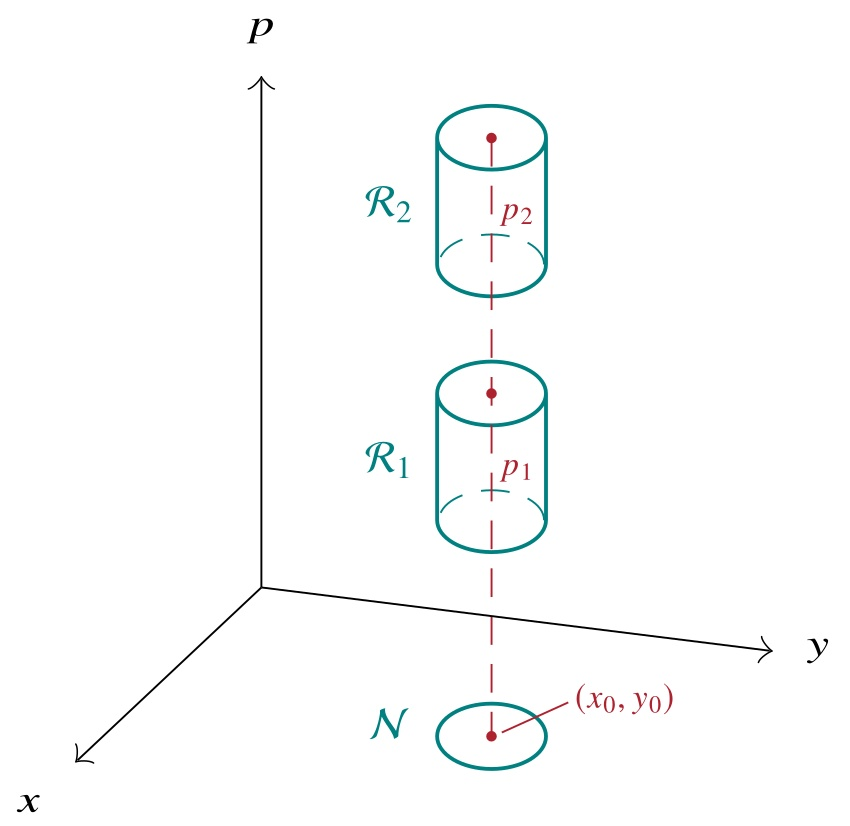
\includegraphics[width=.5\textwidth]{cylinder.jpg}
\caption{Representation of the cylindrical neighbourhoods of each $p_i$ and the projection of every base onto the $(x,y)$-plane.}
\label{fig:cylinder}
\end{figure}

In this situation the implicit function theorem asserts that in each of the cylinders $\mathcal R_i$ (shrunk if necessary) the equation  $F(x,y,p)=0$ is satisfied by one and only one choice of $p$ as a smooth function of $x$ and $y$, that is, of the form
\begin{equation}\label{eq:surface-th}
  p=f_i(x,y), \quad i=1,\dots,m,
\end{equation}
where in each case the derivative with respect to $y$ is given by \eqref{eq:der-formula}. Since $|F_p(x,y,f_i(x,y))| \ge c > 0$ by assumption and given that $F_y$ is continuous, we can assure that each $\partial f_i/\partial y$ is bounded on $\mathcal R_i$.

Not only that, but we can also choose $\mathcal N$ so small that every point $(x,y,p)$ in the cylinder generated by $\mathcal N$ for which $F=0$ belongs to one of the surfaces \eqref{eq:surface-th}. Indeed, if it were not the case, any such point would obviously have to lie outside the cylinders $\mathcal R_1, \dots, \mathcal R_m$, and if they existed for arbitrarily small $\mathcal N$ they would have to be on the line $x=x_0$, $y=y_0$. To see this, we argue by contradiction and suppose that for all $n \in \NN$ there exists a point $(x_n,y_n,p_n) \in G$ with the following properties:

\begin{enumerate}
  \item $F(x_n,y_n,p_n)=0$.
  \item $\lvert (x_n, y_n) - (x_0, y_0)\rvert < \frac{1}{n}$.
  \item $(x_n, y_n, p_n) \in G \setminus \mathcal R$.
\end{enumerate}
Since $G$ is compact, $\{p_n\}$ is bounded, and we can suppose that it converges to some real value $p_0$. Together with property $(ii)$, this information assures that
\[\{(x_n,y_n,p_n)\} \to (x_0,y_0,p_0).
\]
Now, since $G \setminus \mathcal R$ is closed in $G$, $(iii)$ implies that $(x_0,y_0,p_0) \notin \mathcal R$, and in particular that $p_0 \notin \{p_1,\dots,p_m\}$. Finally, by virtue of $(i)$ and the continuity of $F$, we conclude that
\[
0=F(x_n,y_n,p_n) \to F(x_0,y_0,p_0),
\]
meaning that $p_0$ is another root of the equation $F(x_0,y_0,p)=0$, which is impossible since its only roots were $p_1,\dots,p_m$.

Thus we have proven that the point $(x_0,y_0)$ has a neighbourhood $\mathcal N$ where $F(x,y,p)=0$ has precisely $m$ solutions \eqref{eq:surface-th}. Each function $f_i$ is continuous and has a bounded derivative with respect to $y$, so according to Theorem \ref{th:picard} each of the equations
\[
y' =f_i(x,y)
\]
has one and only one integral curve passing through any given point of $\mathcal N$. Repeating the reasoning in the proof of Theorem \ref{th:implicit-basic} we can see that these curves are indeed integral curves of \eqref{eq:implicit-th}. Because the values of $y'$ associated with each integral curve are all different on $\mathcal N$ (since the cylinders $\mathcal R_i$ are disjoint), these integral curves are all different and no two make contact without intersecting. Moreover, if there was another integral curve apart from these ones, its derivative would have to take the values $\overbar{p}_i \in \mathcal R_i$ and $\overbar{p}_j \in \mathcal R_j$ for some $i\neq j$, and by the \textit{intermediate value theorem for derivatives} (see footnote \ref{fn:darboux}) it would have to take every value in between, which is impossible since $F$ only vanishes on $\mathcal R$. Therefore, as asserted, precisely $m$ solutions of equation \eqref{eq:implicit-th} pass through each point of $\mathcal N$.
\end{proof}

A careful look at the statement of this problem reveals that none of the direction fields defined by equation \eqref{eq:implicit-th} can be parallel to the $y$-axis. However, as in the case of equations solved for $y'$, we would like to include this possibility. Therefore, besides the equation
\begin{equation}\label{eq:implicit-again}
  F\left(x,y,\frac{dy}{dx}\right)=0
\end{equation}
we consider the associated equation
\begin{equation}
  \tag{\ref*{eq:implicit-again}'}
  F_1\left(x,y,\frac{dx}{dy}\right)=0,
\end{equation}
where $F_1$ is chosen in such a way that these equations are consistent.

As a final remark, we note that if we could explicitly solve for $y'$ (think for example that $F$ were a polynomial on $y'$) then we could not only establish the existence and uniqueness of solutions, but also determine exactly what those solutions were, as in the next example.

\begin{example} \label{ex:parabolas} Let us revisit the equation
  \begin{equation} \label{eq:ex2}
    (y')^2=y.
  \end{equation}
We know that two direction fields are combined in this equation (see Figure \ref{fig:ex1}), and hence the direction field of \eqref{eq:ex2} is obtained as the superposition of those two direction fields. Setting $F(x,y,p)=p^2-y$ and solving $F=0$ for $p$ yields $p=\pm \sqrt{y}$, for every $y > 0$. We have $F_p=2p$, so we can apply Theorem \ref{th:implicit2} to every point on the set
\[
\{(x,y) \in \R^2: y > 0 \},
\]
obtaining that there is a neighbourhood of each of these points in which there are two and only two integral curves of equation \eqref{eq:ex2} passing through any given point. This is also obvious from Figure \ref{fig:ex1}. What is more, in this case we can obtain an explicit expression of those integral curves by solving the two differential equations
\begin{equation} \label{eq:parabolas}
y'= \pm \sqrt{y}, \quad y > 0,
\end{equation}
whose joint family of solutions can be written as
\[
y(x)=\frac{1}{4}(x+C)^2, \quad C \in \R.
\]
They are convex parabolas with vertex on the $x$-axis, the upwards branch corresponding to the positive sign in \eqref{eq:parabolas} and the downwards branch to the negative sign.
\end{example}

\begin{remark} The above example stresses the importance of working in open sets when it comes to uniqueness of solutions. If we were to solve equation \eqref{eq:ex2} for $y\ge 0$, we would immediately note that the line $y=0$ is an integral curve of the equation, and then an infinite number of solutions would pass through every point on the $x$-axis. In particular, for every $x_0 \in \R$ the functions parametrized by $k\ge x_0$ as
  \[
  \phi_k(x)= \begin{cases}
    0, & x < k,\\
    \frac{1}{4}(x-k)^2, & x \ge k
  \end{cases}
  \]
are all different solutions of the equation passing through the point $(x_0,0)$.

\end{remark}

\section{Geometrical approach to implicit equations}

When studying equations in implicit form, the previous results and techniques suggest a geometrical approach in which we consider the direction field not on the $(x,y)$-plane, but on the surface of the three-dimensional $(x,y,p)$-space given by the equation $F(x,y,p)=0$, where $p=dy/dx$. This way, even though the equation might define several direction fields, we compensate for this by adding a new dimension in which to visualize them together. This space is known as the space of \textit{1-jets} of functions $y(x)$, which is basically representing the truncated Taylor polynomial of a (differentiable) function at a given point. We can regard its points as all the nonvertical directions\footnote{We could circumvent this restriction with the usual trick of considering another function $F_1$, but we will not do it here for simplicity.} (those not parallel to the $y$-axis) at all points of the $(x,y)$-plane: a point $(x,y,p)$ represents the direction of a line $dy=p\,dx$ at the point $(x,y)$. In what follows, the direction of the $p$-axis will be referred to as the \textit{vertical direction}.

For the purposes of this section we will assume that $F$ is a sufficiently differentiable function and that the surface
\[
M = \{ (x,y,p) : F(x,y,p)=0\}
\]
in the space of 1-jets is smooth\footnote{This is not a strong restriction, since it holds if $0$ is not a critical value of $F$, and by Sard's theorem this happens almost always. Even if it were not the case, a small perturbation by an additive constant should make it so.}. We will show that a direction field arises on this surface and relate it to a certain direction field on the plane. Before we continue, we define a concept that will be essential in the development of the theory.

\begin{definition}
A point on the surface $M$ is called a \textit{regular point} if the tangent plane to the surface at that point is not vertical.
\end{definition}
Let us recall that the tangent plane at a point $(x_0,y_0,p_0)$ of the surface $M$ is given by the equation
\begin{equation} \label{eq:tangent}
\langle \nabla F(x_0,y_0,p_0), (x-x_0,y-y_0,p-p_0) \rangle = 0,
\end{equation}
so that it is nonvertical if and only if $F_p(x_0,y_0,p_0) \neq 0$. This condition should look familiar after seeing the results of the previous section. Let
\[
\pi:M\to\R^2, \quad \pi(x,y,p)=(x,y)
\]
be the projection of $M$ to the $(x,y)$-plane in the vertical direction. A \textit{critical point} of the mapping $\pi$ will be a point for which $F=F_p =0$, that is, a point on $M$ that is not regular.

Thus, in a neighbourhood of a regular point we can apply yet again the implicit function theorem to show that $M$ is the graph of a smooth function, say $p=f(x,y)$. In fact, it is a well-known result in the basic theory of differentiable surfaces that in this case the projection $\pi$ is a local diffeomorphism (see \cite[39]{montiel2009curves}). Then, to each regular point corresponds its own differential equation (in a neighbourhood of the projection of said point) and the direction field that comes with it; all these direction fields on the $(x,y)$-plane are combined in the equation $F=0$.

On the other hand, we forget the projection momentarily and consider a point $(x,y,p)$ in the space of 1-jets and a vector $\xi$ applied at this point, whose components will be denoted by $dx(\xi)$, $dy(\xi)$ and $dp(\xi)$. We now consider the plane of all such vectors at a point $(x,y,p)$ for which $dy=p\,dx$\footnote{In differential geometry this is known as (the kernel of) a 1-form.}, that is, the vectors that when projected onto the $(x,y)$-plane form an angle  with the $x$-axis whose tangent is equal to $p$. Each of these planes is called a \textit{contact plane}, and they are all vertical (they contain the direction of the $p$-axis, since the vector $(0,0,1)$ verifies the condition imposed). The set of all contact planes forms the \textit{contact plane field} in the space of jets, and is called the \textit{contact structure}\footnote{This term is not specific to this problem, but is an important notion in a branch of geometry known as contact geometry, which falls outside of the scope of this work.}. Figure \ref{fig:jets} can help visualize the various elements of this construction.

\begin{figure}[h!]
\centering
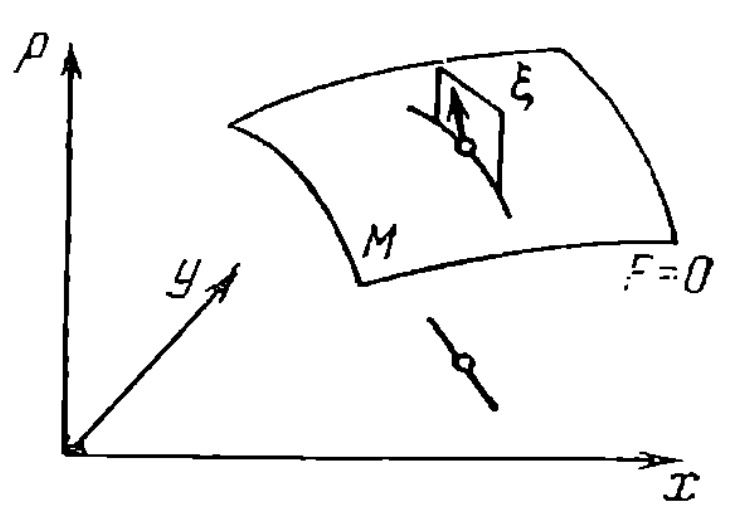
\includegraphics[width=.4\textwidth]{jets.jpg}
\caption{The surface $M$, the contact plane at a point and its projection. Taken from \cite{arnold2012geometrical}.}
\label{fig:jets}
\end{figure}

Bringing back the projection, we study the contact plane at a regular point of the surface $M$. Since the contact plane is vertical, it intersects the corresponding tangent plane in a line, and this behaviour is reproduced in all the nearby points. In this way, in a neighbourhood of a regular point there arises a smooth direction field, given by the intersections of the contact and tangent planes at every point. The integral curves of equation \eqref{eq:ode-implicit} are, by definition, the integral curves of this direction field on $M$. We can even provide an explicit description of this direction field by analyzing the intersection of the two planes. Firstly, since the contact plane at a regular point $(x,y,p)$ is given by the equation $p\,dx - dy = 0$, the normal vector to this plane at the point $(x,y,p)$ is $(p,-1,0)$, and secondly we know by equation \eqref{eq:tangent} that the normal vector to the tangent plane at said point is $\nabla F(x,y,p)$. Then, the line resulting from the intersection of both planes at the point of interest is given by the direction
\[
\nabla F(x,y,p) \times (p,-1,0) = {(F_p, pF_p, - (F_x+pF_y))\,}_{\mkern 1mu \vrule width 0.75pt height 2ex\mkern2mu \,(x,y,p)},
\]
and thus the direction field on $M$ is defined by the vector field
\begin{equation} \label{eq:field}
V = (F_p, pF_p, -(F_x+pF_y)).
\end{equation}

We are now ready to link these seemingly distinct direction fields (the one on $M$ and the ones on the $(x,y)$-plane we mentioned earlier), though it should be clear by now what the conclusion will be: that the direction field on $M$ projects locally onto a direction field on the plane.

\begin{theorem}
  The vertical projection onto the $(x,y)$-plane in the neighbourhood of a regular point maps integral curves of equation \eqref{eq:ode-implicit} on $M$ into integral curves of the equation
  \begin{equation} \label{eq:implicit-graph}
      \frac{dy}{dx}=f(x,y)
  \end{equation}
  in a neighbourhood of the projection of the point under consideration. Here $f$ is a smooth function such that $M$ is locally the graph of $f$.
\end{theorem}

\begin{proof}
We know by definition that the projection of a contact plane onto the $(x,y)$-plane is a straight line in the direction field of equation \eqref{eq:implicit-graph}, because it holds that $p=f(x,y)$. Then, since $\pi$ is a diffeomorphism in the neighbourhood considered, the direction field on $M$ turns into the direction field of \eqref{eq:implicit-graph}. Consequently, the integral curves turn into each other, as well.
\end{proof}

The conclusion we can extract from all this reasoning is that, in the neighbourhood of a regular point, an implicit equation can be turned into an explicit one and can be studied and solved with the usual methods. However, special attention should be paid to critical points, that is, points in which the equation does not reduce to an explicit one, and in fact we will expand on this matter in the next section. For now, we define a couple of concepts related to these points, and we bring this section to an end with an example.

\begin{definition} The set $C$ of critical points of the projection $\pi$ is called the \textit{criminant curve} of equation \eqref{eq:ode-implicit}, and the set $\pi(C)$ of its images is called the \textit{discriminant curve}.
\end{definition}

\begin{remark} The discriminant curve can be obtained in some cases by eliminating $p$ in the equations $F=F_p=0$.

\end{remark}

\begin{example} \label{ex:cusp}
  We want to study the equations $p^2=x$ and $p^2=y$ using the techniques of this section. For the first one, we write down the equations of a generic vector at a point $(x,y,p)$ on $M$ that belongs to the direction field:
  \[
  \begin{cases}
    p^2=x & \text{(the condition of belonging to $M$)},\\
    2p\,dp=dx & \text{(the condition of being tangent to $M$)},\\
    dy=p\,dx & \text{(the condition of belonging to the contact plane)}.
  \end{cases}
  \]
We note that the criminant is given by the curve $p=0$ on $M$, which results when projected in a disciminant curve consisting on the $x$-axis (it follows from the first condition that $x=0$ when $p=0$). In this case it is convenient to choose the coordinates $(p,y)$ on $M$. Combining the conditions above we get that (in our chosen coordinates) the integral curves are defined by the equation
\[
\frac{dy}{dp} = 2p^2,
\]
which we can easily solve to get that the solutions are given by the relation $y+C=\frac{2}{3}p^3$. Projecting back to the $(x,y)$-plane yields integral curves defined parametrically by
\[
x=p^2, \quad y= \frac{2}{3}p^3 + C, \quad C \in \R.
\]
If we want, we can also reverse the change of variables to write down the solutions as a more direct relation between $x$ and $y$:
\[
(y+C)^2 = \frac{4}{9}p^6 \implies (y+C)^2 = \frac{4}{9}x^3,\quad C \in \R.
\]
It can be checked that these solutions are semicubical parabolas with a cusp on the discriminant line $x=0$, as seen in Figure \ref{fig:parabola}.

\begin{figure}[h!]
\centering
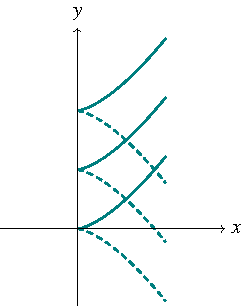
\includegraphics[height=17em]{parabola}
\caption{Integral curves of the equation $p^2=x$ on the plane.}
\label{fig:parabola}
\end{figure}

The other equation $p^2=y$ is solved in a similar way. The conditions in this case are the following:

  \[
  \begin{cases}
    p^2=y,\\
    2p\,dp=dy,\\
    dy=p\,dx.
  \end{cases}
  \]
The criminant is again $p=0$, but in this case the discriminant curve is the $x$-axis. If we choose coordinates $(x,p)$ on $M$ the resulting equation outside of the criminant is
\[
\frac{dx}{dp}=2,
\]
which yields solutions of the form
\[
x=2p + C, \quad y=p^2, \quad C \in \R,
\]
or equivalently,
\[
(x+C)^2=4y, \quad C \in \R.
\]
\end{example}
These are parabolas tangent to the line $y=0$, as we already knew from Example \ref{ex:parabolas}.

\section{Singular points and singular solutions}

Another common terminology for referring to the points on the criminant curve is to call them \textit{singular points} of the equation $F=0$. It is worth pointing out that at some singular points it may well be the case that the contact plane is different from the tangent plane, so that they intersect in a straight line and thus still produce a direction field. In fact, we can extend the direction field defined in the previous section to include these well-behaved points, and say that this extended field is the \textit{direction field of the equation $F=0$ on $M$}. However, at singular points the conditions to apply the implicit function theorem do not hold (we have $F_p=0$), so we can only assure that projections of the pieces of the integral curves (of the extended field) localized between singular points are locally integral curves of the corresponding equations $y'=f(x,y)$.

Following the distinction outlined above between singular points, and remembering the expression \eqref{eq:field} for the direction field on $M$, we arrive at the following definition.

\begin{definition}
  A singular point of equation $F=0$ (a point on $M$ for which $F_p=0$) is called a \textit{proper singular point} if $F_x+pF_y \neq 0$, and an \textit{improper singular point} otherwise.
\end{definition}
In the first case, if $(x_0,y_0,p_0)$ is a proper singular point, the tangent and contact planes intersect each other at the straight line passing through $(x_0,y_0,p_0)$ and having direction
\[
v=(0,0,-F_x(x_0,y_0,p_0)-p_0F_y(x_0,y_0,p_0)).
\]
In the second case, the contact and tangent planes coincide at the point $(x_0,y_0,p_0)$ and no straight line is produced. Now, among proper singular points we distinguish those which verify an additional smoothness condition: we will refer by \textit{regular singular point}\footnote{Not to be confused with a regular point of $\pi$.} or \textit{folded proper point} to a proper singular point that verifies
\[
\operatorname{rank}((x,y,p) \mapsto (F,F_p)) = 2,
\]
where the rank of a mapping is defined as the rank of its derivative (which is a linear map). Note that this condition guarantees via the implicit function theorem that the criminant curve is a smooth curve. Moreover, almost all singular points are of this type, by virtue of Sard's theorem (cf. \cite[94]{arnold2012geometrical}).

It turns out that at every regular singular point, the equation $F=0$ is equivalent to another equation of the form $p^2=x$ for a suitable change of coordinates. This is what is called the \textit{normal form} of the equation $F=0$.

\begin{theorem}[Normal form] Let $(x_0,y_0,p_0)$ be a regular singular point of the equation $F(x,y,p)=0$. Then, there exists a diffeomorphism of a neighbourhood of the point $(x_0,y_0)$ in the $(x,y)$-space to a neighbourhood of the point $(0,0)$ in the $(X,Y)$-space such that the equation $F=0$ is reduced to the form $P^2=X$, where $P=dY/dX$.

\end{theorem}

\begin{proof}
  A detailed proof can be found in \cite[27]{arnold2012geometrical}, which in turn is based on the original 1932 article by Italian mathematician M. Cibrario \cite{cibrario1932reduzione}.
\end{proof}
If we revisit Example \ref{ex:cusp} we realize that the equation in normal form can easily be solved, so the following result is immediate.

\begin{corollary} In a neighbourhood of a regular singular point, the family of solutions of the equation $F=0$ is diffeomorphic to the family of semicubical parabolas $y=x^{3/2}+C$.

\end{corollary}

The previous corollary allows us to call these singularities \textit{cusp singularities}. We note that another type of singularities may arise in the discriminant curve, since in general several points of the criminant curve may be mapped by $\pi$ onto the same point in the discriminant curve. These points will almost always be points of self-intersection of the discriminant curve, and they are called \textit{fold singularities}. There are even more types of singularities that we could encounter, but a result by Whitney \cite{whitney1955singularities} states that for an open dense set of functions $F$, the projection $\pi$ is either a local diffeomorphism, a fold map or a cusp map at every point. That is to say, if a function presents another type of singularity, almost every small perturbation would eliminate them. Nevertheless, some attempts have been made at a classification of singularities of implicit equations; see \cite{chertovskih2014pleated} or \cite{dara1975singularites}.

Finally, we explore the concept of singular solutions. A \textit{singular solution} of equation $F=0$ is a solution of the equation that is composed entirely of (projections of) singular points. Such solutions are special because they usually cannot be found as part of the general solution. More explicitly, if we have a parametrized family of solutions

\begin{equation} \label{eq:envelope}
  \Phi(x,y,C)=0,
\end{equation}
generally there is no value of $C$ such that when substituted in \eqref{eq:envelope} a singular solution is obtained. For example, equation $p^2=x$ in Example \ref{ex:parabolas} presented a singular solution consisting on the line $x=0$, which happens to be tangent at each point to the family of semicubical parabolas found as ``regular'' solutions. It turns out that this situation is not exceptional, and that most singular solutions occur in this way, so that the following definition is relevant\footnote{A study on the relation between singular solutions and envelopes was started by Darboux in 1873 \cite{darboux1873solutions}.}.

\begin{definition}An \textit{envelope} of a family of plane curves is a curve that is tangent to each member of the family at some point, and these points of tangency together form the whole envelope.

\end{definition}

\begin{remark} It is obvious from the tangency condition that the envelope of a family of solutions to $F=0$ is itself a solution. Moreover, at any point $(x_0,y_0)$ of the envelope there are two solutions of the equation passing through it with the same slope $p_0$: the curve of the underlying family that is tangent to the envelope at that point and the envelope itself. Then we have necessarily that $F_p(x_0,y_0,p_0)=0$, for if this were not the case it would contradict the uniqueness in Theorem \ref{th:implicit-basic}. Thus we conclude that an envelope of a family of solutions to $F=0$ is always a singular solution of that equation.
\end{remark}

However, not every family of curves has an envelope. The following result provides some necessary conditions for this to happen, and in practice it gives us a method to find envelopes.

\begin{theorem}
If a family of curves $\Phi(x,y,C)=0$ has an envelope, then the points of the envelope must simultaneously satisfy the equations $\Phi = \Phi_C=0$.
\end{theorem}

\begin{proof}
Since the envelope is tangent to each member of the family of curves at some point, we can regard it as a map from the parameter $C$ to the point of tangency. That is, we can write the points of the envelope as $x=x(C)$, $y=y(C)$. Since the envelope meets every curve of the family, it holds that
 \[
\Phi(x(C),y(C),C)=0, \quad \text{for all } C,
 \]
which is the first equation claimed to be satisfied by the envelope. Moreover, taking the derivative with respect to $C$ in the previous expression and applying the chain rule yields
\begin{equation} \label{eq:envelope1}
  \Phi_x \frac{dx}{dC} + \Phi_y \frac{dy}{dC} + \Phi_C = 0.
\end{equation}
 On the other hand, the slope of the envelope at any point is given by
 \begin{equation} \label{eq:envelope2}
   \frac{dy}{dx} = \frac{dy/dC}{dx/dC},
 \end{equation}
and we can also take a particular curve and differentiate $\Phi(x,y,C)$ with respect to $x$ (with $C$ is held constant), getting that the slope at any point of that curve is expressed as
\begin{equation} \label{eq:envelope3}
\Phi_x + \Phi_y \frac{dy}{dx} = 0.
\end{equation}
Now, since for a fixed $C$ the envelope is tangent to the curve $\Phi(x,y,C)=0$ at $(x(C),y(C))$, we can combine \eqref{eq:envelope2} and \eqref{eq:envelope3} to get
\[
\Phi_x \frac{dx}{dC} + \Phi_y \frac{dy}{dC} = 0,
\]
which in light of \eqref{eq:envelope1} implies that $\Phi_C=0$ at every point of the envelope, as asserted.
\end{proof}

If we want to find an envelope for a given family of curves $\Phi$, attending to the result just proved we could try to eliminate $C$ from the equations $\Phi=\Phi_C=0$ and check that the resulting curve verifies the conditions of an envelope. Even though this is the most common method to find envelopes, it is also interesting to analyze what are the sufficient conditions for their existence, to which the following theorem (proved in \cite[10]{burns1961envelopes}) gives a complete answer.

\begin{theorem} \label{th:sufficient} If $\Phi(x,y,C)$ is a twice-differentiable function satisfying
  \begin{enumerate}
    \item $\Phi=\Phi_C=0$.
    \item $\Phi_{CC}\neq 0$.
    \item $\begin{vmatrix} \Phi_x & \Phi_y\\
                    \Phi_{Cx} & \Phi_{Cy}\end{vmatrix} \neq 0$,
  \end{enumerate}
  then there exists an envelope of the family of functions represented by $\Phi$.

\end{theorem}

\begin{example} Let us consider the differential equation
  \begin{equation} \label{eq:example-envelope}
    1 + (y')^2 = \frac{1}{y^2}.
  \end{equation}
  The change of variables $t=1-y^2$ and a direct integration in both branches of the equation yields the family of solutions
  \begin{equation} \label{eq:circles-envelope}
  \Phi(x,y,C) = (x+C)^2 + y^2 -1 = 0, \quad C \in \R,
\end{equation}
  which are circles of radius 1 and center on the $x$-axis. To find the potential envelope, we differentiate this equation with respect to $C$, getting
  \[
  \Phi_C(x,y,C) = 2(x+C)=0,
  \]
  which combined with $\Phi=0$ implies that $y=\pm 1$. It is clear that the lines $y=1$ and $y=-1$ are both tangent to the family \eqref{eq:circles-envelope}, as seen in Figure \ref{fig:envelope}, so they are indeed the envelopes of the equation \eqref{eq:example-envelope}. We can also check that these lines form the discriminant of the equation, since $F_p=2p$ only vanishes at $p=0$, which by \eqref{eq:example-envelope} implies that $y=\pm 1$. Thus, we have found two singular solutions of the equation, and besides, they constitute the envelopes of the family of general solutions.
\begin{figure}[h!]
\centering
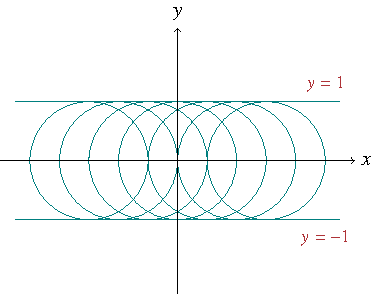
\includegraphics[width=.6\textwidth]{envelope}
\caption{Representation of the family of general solutions of equation \eqref{eq:example-envelope} and its envelopes $y=\pm 1$.}
\label{fig:envelope}
\end{figure}
\end{example}

\begin{example} A classical counterexample to the existence of envelopes is the family of concentric circles at the origin, described by the equation
  \[
  \Phi(x,y,C)=x^2+y^2 -C^2 =0.
  \]
If we tried the usual trick of eliminating $C$ from $\Phi=\Phi_C=0$ we would end up with the equation $x^2+y^2=0$, which in fact is satisfied only by the point $(0,0)$, and thus does not constitute a curve, much less a curve tangent to the family of solutions. A look at Theorem \ref{th:sufficient} tells us that this family does indeed have no envelope, since condition $(iii)$ does not hold at any point. This is also obvious from Figure \ref{fig:concentric}.
\begin{figure}[h!]
\centering
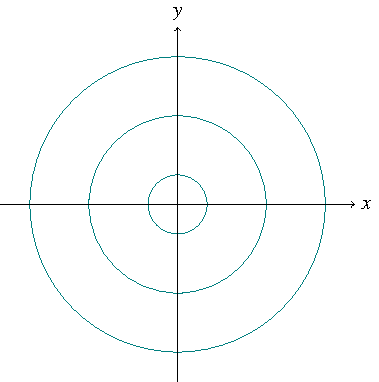
\includegraphics[width=.5\textwidth]{concentric}
\caption{Representation of a family of curves with no envelope.}
\label{fig:concentric}
\end{figure}
\end{example}



%%%% End part
\bookmarksetup{startatroot}% this is it
\addtocontents{toc}{\bigskip}% perhaps as well

%%% Acronyms
% Abkürzungsverzeichnis
\printnoidxglossaries
\addcontentsline{toc}{chapter}{Acronyms}
\cleardoublepage

%%%%%%%%%%%%%%%%%%%%%%%%%%%%%%%%%%%%%%%%%%%%%%%%%%%%%%%%%%%%%%%%%%%%%%%%%%%%%%
%
% Bibliography
%
%%%%%%%%%%%%%%%%%%%%%%%%%%%%%%%%%%%%%%%%%%%%%%%%%%%%%%%%%%%%%%%%%%%%%%%%%%%%%%


%\nocite{*}
\printbibliography

\noindent All links were last followed on September 7, 2020.


\end{document}
